% !Mode:: "TeX:UTF-8"
%%%%%%%%%%%%%%%%%%%%%%%%%%%%%%%%%%%%%%%%%%%%%%%%%%%%%%%%%%%%%%%%%%%%%%%%%%%%%%%%
%          ,
%      /\^/`\
%     | \/   |                CONGRATULATIONS!
%     | |    |             SPRING IS IN THE AIR!
%     \ \    /                                                _ _
%      '\\//'                                               _{ ' }_
%        ||                     hithesis v3                { `.!.` }
%        ||                                                ',_/Y\_,'
%        ||  ,                   dustincys                   {_,_}
%    |\  ||  |\          Email: yanshuoc@gmail.com             |
%    | | ||  | |            https://yanshuo.name             (\|  /)
%    | | || / /                                               \| //
%    \ \||/ /       https://github.com/dustincys/hithesis      |//
%      `\\//`   \\   \./    \\ /     //    \\./   \\   //   \\ |/ /
%     ^^^^^^^^^^^^^^^^^^^^^^^^^^^^^^^^^^^^^^^^^^^^^^^^^^^^^^^^^^^^^^
%%%%%%%%%%%%%%%%%%%%%%%%%%%%%%%%%%%%%%%%%%%%%%%%%%%%%%%%%%%%%%%%%%%%%%%%%%%%%%%%
\documentclass[type=bachelor]{hithesisbook}
% 此处选项中不要有空格
%%%%%%%%%%%%%%%%%%%%%%%%%%%%%%%%%%%%%%%%%%%%%%%%%%%%%%%%%%%%%%%%%%%%%%%%%%%%%%%%
% 必填选项
% type=doctor|master|bachelor|postdoc
%%%%%%%%%%%%%%%%%%%%%%%%%%%%%%%%%%%%%%%%%%%%%%%%%%%%%%%%%%%%%%%%%%%%%%%%%%%%%%%%
% 选填选项(选填选项的缺省值已经尽可能满足了大多数需求,除非明确知道自己有什么
% 需求)
% campus=shenzhen|weihai|harbin
%   含义:校区选项,默认harbin
% glue=true|false
%   含义:由于我工规范中要求字体行距在一个闭区间内,这个选项为true表示tex自
%   动选择,为false表示区间内一个最接近版心要求行数的要求的默认值,缺省值为
%   false。
% tocfour=true|false
%   含义:是否添加第四级目录,只对本科文科个别要求四级目录有效,缺省值为
%   false
% fontset=windows|mac|ubuntu|fandol|adobe
%   含义:设置字体,默认情况会自动识别系统,然后设置字体。后两个是开源字体,自行
%   下载安装后设置使用。windows是中易字库,窝工默认常用字体,绝对没毛病。mac和
%   ubuntu 默认分别是华文和思源字库,理论上用什么字库都行。后两种开源字库的安装
%   方法到谷歌上百度一下什么都有了。Linux非ubuntu发行版、非x86架构机器等如何运行
%   可到github issue上讨论。
% tocblank=true|false
%   含义:目录中第一章之前,是否加一行空白。缺省值为true。
% chapterhang=true|false
%   含义:目录的章标题是否悬挂居中,规范中要求章标题少于15字,所以这个选项
%   有无没什么用,除了特殊需求。缺省值为true。
% fulltime=true|false
%   含义:是否全日制,缺省值为true。非全日制如同等学力等,要在cover中设置类
%   型,封面中不同格式
% subtitle=true|false
%   含义:论文题目是否含有副标题,缺省值为false,如果有要在cover中设置副标
%   题内容,封面中显示。
% newgeometry=one|two
%   含义:规范中的自相矛盾之处,版芯是否包含页眉页脚,旧方法是按照包含页眉
%   页脚来设置。该选项是多选选项,如果没有这个选项,缺省值是旧模板的版芯设
%   置方法,如果设置该选项one或two,分别对应两种页眉页码对应版芯线的相对位
%   置。第一种是严格按照规范要求,难看。第二种微调了页眉页码位置,好一点。
% debug=true|false
%   含义:是否显示版芯框和行号,用来调试。默认否。
% openright=true|false
%   含义:博士论文是否要求章节首页必须在奇数页,此选项不在规范要求中,按个
%   人喜好自行决定。 默认否。注意,窝工的默认情况是打印版博士论文要求右翻页
%   ,电子版要求非右翻页且无空白页。如果想DIY(或身不由己DIY)在什么地方右
%   翻页,将这个选项设置为false,然后在目标位置添加`\cleardoublepage`命令即
%   可。
% library=true|false
%   含义:是否为提交到图书馆的电子版。默认否。注意:如果设置成true,那么
%   openright选项将被强制转换为false。
% capcenterlast=true|false
%   含义:图题、表题最后一行是否居中对齐(我工规范要求居中,但不要求居中对
%   齐),此选项不在规范要求中,按个人喜好自行决定。默认否。
% subcapcenterlast=true|false
%   含义:子图图题最后一行是否居中对齐(我工规范要求居中,但不要求居中对齐
%   ),此选项不在规范要求中,按个人喜好自行决定。默认否。
% absupper=true|false
%   含义:中文目录中的英文摘要在中文目录中的大小写样式歧义,在规范中要求首
%   字母大写,在work样例中是全大写。该选项控制是否全大写。默认否。
% bsmainpagenumberline=true|false
%   含义:由于本科生论文官方模板的页码和页眉格式混乱,提供这个选项自定义设
%   置是否在正文中显示页码横线,默认否。
% bsfrontpagenumberline=true|false
%   含义:由于本科生论文官方模板的页码和页眉格式混乱,提供这个选项自定义设
%   置是否在前文中显示页码横线,默认否。
% bsheadrule=true|false
%   含义:由于本科生论文官方模板的页码和页眉格式混乱,提供这个选项自定义设
%   置是否显示页眉横线,默认显示。
% splitbibitem=true|false
%   含义:参考文献每一个条目内能不能断页,应广大刀客要求添加。默认否。
% newtxmath=true|false
%   含义:数学字体是否使用新罗马。默认是。
% chapterbold=true|false
%   含义:本科生章标题在目录和正文中是否加粗
%%%%%%%%%%%%%%%%%%%%%%%%%%%%%%%%%%%%%%%%%%%%%%%%%%%%%%%%%%%%%%%%%%%%%%%%%%%%%%%%
\usepackage{hithesis}
\usepackage{url}


%%%%%%%%%%%%%%%%%%%%%%%%%%%%%%%%%%%%%%%%%%%%%%%%%%%%%%%%%
\usepackage{listings}
\lstset{
	language=C,
	keywordstyle=\color{blue!70},
	basicstyle=\small\ttfamily,
	numbers=left,
	numberstyle=\tiny,
	frame=tb,
	columns=fullflexible,
	showstringspaces=false
}
\renewcommand\lstlistingname{代码}
\renewcommand\lstlistlistingname{代码}
%%%%%%%%%%%%%%%%%%%%%%%%%%%%%%%%%%%%%%%%%%%%%%%%%%%%%%%%%


\graphicspath{{figures/}}
\begin{document}
\frontmatter
% !Mode:: "TeX:UTF-8"

\hitsetup{
  %******************************
  % 注意:
  %   1. 配置里面不要出现空行
  %   2. 不需要的配置信息可以删除
  %******************************
  %
  %=====
  % 秘级
  %=====
  statesecrets={公开},
  natclassifiedindex={TM301.2},
  intclassifiedindex={62-5},
  %
  %=========
  % 中文信息
  %=========
  ctitleone={\large{基于C语言的RISC-V}},%本科生封面使用
  ctitletwo={\large{操作系统设计与实现}},%本科生封面使用
  ctitlecover={基于C语言的RISC-V操作系统设计与实现},%放在封面中使用,自由断行
  ctitle={基于C语言的RISC-V操作系统设计与实现},%放在原创性声明中使用
  % csubtitle={一条副标题}, %一般情况没有,可以注释掉
  cxueke={工学},
  csubject={计算机科学与技术},
  caffil={计算学部},
  cauthor={郭子阳},
  csupervisor={刘国军},
  % 日期自动使用当前时间,若需指定按如下方式修改:
  %cdate={2021年6月1日},
  cstudentid={1170300520},
  cnumber={no9527}, %编号
  %=========
  % 英文信息
  %=========
  etitle={Design and implementation of a C-based RISC-V operating system},
  % esubtitle={This is the sub title},
  exueke={Engineering},
  esubject={Computer Science and Technology},
  eaffil={\emultiline[t]{School of Computer Science \\ and Engineering}},
  eauthor={Guo Ziyang},
  esupervisor={Liu Guojun},
  % 日期自动生成,若需指定按如下方式修改:
  % edate={December, 2017},
  % estudenttype={Master of Art},
  %
  % 关键词用“英文逗号”分割
  ckeywords={RISC-V, 操作系统, 内存管理,ELF文件, 文件系统, 壳(shell)},
  ekeywords={RISC-V, operating system, memory management, ELF file, file system, shell},
}

\begin{cabstract}

指令集架构(ISA)是计算机的一种抽象模型,是计算机体系结构模型中与程序设计相关的部分,也是处理器的灵魂。现阶段市场上常见的ISA,如x86和ARM,都是商业闭源的,不利于二次开发。于是RISC-V一出现,就受到了各大研究机构和高校的青睐。同样,这款完全开源的指令集架构,也有助于解决我国当前面临的芯片困境,进一步反哺国内生态,尤其是操作系统方面,以保障我国在核心产业的自主可控。

尽管RISC-V已经出现多年,国内对它的研究却一直局限于嵌入式和移动设备领域,同时,对于RISC-V指令集架构的通用操作系统的研究,相关资料较少且专业性过强,成为阻碍其进入高校研究和课堂教学的重要因素。

为了解决上述问题,进一步推动RISC-V在高校教学中的沉淀,促进RISC-V的传播,本论文讨论了一种基于C语言的RISC-V操作系统的设计,基于模块对整个工程进行划分,随后进一步细化了各个模块的具体设计,譬如中断的模式、线程调度算法等,并主要给出各个模块的实现细节,最后针对此操作系统,给出了一份比较详细的实现文档。本文实现的操作系统主要分为四个模块:中断管理、内存管理、线程调度和文件系统。中断模块主要用于处理环境调用,同时处理定时器中断来辅助线程调度;内存管理模块对操作系统的可用物理内存进行管理分配,内存管理以两个粒度进行:动态内存分配和按页分配,并实现虚拟内存以进行进程间的代码数据隔离;线程调度保证了所有正在运行的线程都有平等使用CPU的机会,并根据需要动态挂起和唤醒线程;文件系统对操作系统开放了一个统一的文件读写接口,使得不同类型的文件实现细节对操作系统来说是透明的。

本文设计实现的基于C语言的RISC-V操作系统,结构清晰,方便横向扩展。同时代码规范,注释和文档完整详细,可用于教学用途,并可以在客观上推动RISC-V开源社区的发展。

\end{cabstract}

\begin{eabstract}

Instruction Set Architecture (ISA) is an abstract model of computer, a part of computer architecture model related to programming, and also the soul of the processor. Currently, common ISA such as x86 and ARM, are commercial closed source, which is not conducive to secondary development. As soon as RISC-V appeared, it was favored by various research institutions and universities. In the same way, this completely open source instruction set architecture will also help solve China's current chip dilemma and further feed the domestic ecology, especially in the aspect of operating system, so as to guarantee China's autonomy and control in the core industry.

Although RISC-V has been brought up for many years, domestic research on RISC-V has been limited to the field of embedded and mobile devices. At the same time, for the research on RISC-V general operating system, there are few relevant materials and it is too specialized, which has become an important factor hindering its entry into university research and classroom teaching.

In order to solve the above problems, further promote the participation of RISC-V in college teaching and promote the spread of RISC-V, this paper discusses a RISC-V operating system based on C language design. This paper first divides the whole project based on modules, then further discusses the specific design of each module, such as interrupt mode, thread scheduling, etc., and gives the implementation details of each module. Finally, a detailed implementation document is given for this operating system. The operating system realized in this paper is mainly divided into four modules: interrupt management, memory management, thread scheduling and file system. The interrupt management module is mainly used to handle the environment call and timer interrupt to assist thread scheduling. The memory management module manages and allocates the physical memory the system can use. The memory management is carried out in two granularity: dynamic memory allocation and page-based allocation, and the virtual memory is realized to isolate the code and data between processes. Thread scheduling ensures that all running threads have equal access to CPU, and dynamically suspends and awakens threads as needed. The file system provides a unified file reading and writing interface to the operating system, making the implementation details of different types of files transparent to the operating system.

The RISC-V operating system based on C language designed and implemented in this paper has a clear structure and is convenient for horizontal expansion. At the same time, the code conforms to the specification, the comments and documentation are comprehensive and detailed, so as to be used for educational purposes. And it can objectively promote the development of RISC-V open source community.

\end{eabstract}
 % 封面
\makecover
%\begin{denotation}
\begin{table}[h]%此处最好是h
\caption{国际单位制中具有专门名称的导出单位}
\vspace{0.5em}\centering\wuhao
\begin{tabular}{ccccc}
\toprule[1.5pt]
量的名称&单位名称&单位符号&其它表示实例\\
\midrule[1pt]
频率&赫[兹]&Hz&s-1\\
\bottomrule[1.5pt]
\end{tabular}
\end{table}
\end{denotation}
%物理量名称表,符合规范为主,有要求添加
\tableofcontents %目录
\mainmatter
% !Mode:: "TeX:UTF-8"

\chapter{绪论}[Introduction]

\section{课题来源及研究的目的和意义}

指令集架构(ISA),是计算机的一种抽象模型,是计算机体系结构模型中与程序设计相关的部分。通常,指令集架构定义了一系列支持的数据类型、寄存器、内存管理、基本特性与IO模型。计算机处理器的指令集架构有以下常见的两种:复杂指令集架构(CISC)、精简指令集架构(RISC),前者的代表就是x86架构,而后者的代表就是ARM架构。无论如何划分,不可否认的是,当今最流行的几个指令集架构,如x86和ARM,都是商业闭源的,在使用这些指令集架构时,需要向Intel或ARM控股缴纳高额的许可费。但是,Krste Asanović等人提出了这样一个观点:指令集架构应当是开放的,并以RISC-V作为开源指令集架构的典型进行论述。

RISC-V是一个基于精简指令集原则的开源指令集架构,该项目2010年始于加州大学伯克利分校,但是该项目的贡献者更多的是校外的志愿者和行业工作者。尽管不是第一个开源指令集,但是由于RISC-V适用于各种设备,譬如云计算机、PC机、移动设备和嵌入式系统,且其开源免费的特性使得它的社区十分活跃。于是RISC-V架构一经出现,就有许多芯片设计者以此为架构设计SoC。

相较于以功耗低著称的ARM架构处理器,RISC-V性能更强、面积更小、功耗更低,且相对于ARM,指令更加丰富,可扩展性更强,并且开源免费。或许是感受到了来自RISC-V的巨大压力,ARM控股甚至上线了一个网站来专门质疑RISC-V指令集。而相对于Intel的x86指令集架构,RISC-V没有那么多的历史包袱,不需要考虑向后兼容问题,可以说是“轻装上阵”,在设计操作系统时就无须考虑类似“A20地址线”的问题。而在关键技术被其他国家卡脖子的当今中国,开源免费的RISC-V可能有助于我国打破芯片壁垒。

同时,随着我国逐渐重视核心技术国有化,保障我国核心产业自主可控,我国开始大力发展自研芯片和自研操作系统。然而,相关工作大都是在企业和研究院层面展开,并没有下沉到高校层面的,形成了产学断层。这使得对于RISC-V相关技术的研究和教学,如RISC-V架构的芯片和支持RISC-V的操作系统的相关方向,成为国内高校研学的一片空白地带。

目前,大部分高校的操作系统的课程,都是基于x86架构设计的。然而,x86架构向后兼容的特性,使得即使是较新的x86操作系统,也不得不兼容一些过时的、已经被废弃不用的特性,例如上文提到的A20地址线。这使得学生对于操作系统本身的概念,会和x86一些特性混淆。令学生可能会更专注于繁琐而多余的x86特性,而不是聚焦于操作系统领域的通用概念。而RISC-V架构的操作系统,由于架构本身的精巧轻盈,更能让学生着眼于系统自身的设计。

基于以上原因,本文讨论了一种基于C语言和RISC-V架构的操作系统的设计方案,并给出其实现代码,旨在推动RISC-V向高校课程和实验室的下沉,以期能够反哺开源社区,最终客观上促进社区发展和RISC-V在国内的传播。

\section{国内外研究现状及分析}

\section{研究内容与方案}
% !Mode:: "TeX:UTF-8"

\chapter{RISC-V相关硬件机制}[riscv]
\label{chapter:riscv}
% !Mode:: "TeX:UTF-8"

\chapter{系统整体设计}[overall]
\label{chapter:overall}

本章简明描述本文所设计的操作系统的体系结构和主要的构成模块,旨在对整个操作系统有一个整体的把握。目前暂时将这个操作系统命名为“Moonix”,后文中的“Moonix”皆指本文所设计实现的操作系统。

目前,整个Moonix操作系统设计有两个部分组成:监管者模式部分和用户模式部分。监管者模式部分即操作系统内核,用于对硬件资源进行抽象和调度访问,向下沟通位于机器模式的SBI,向上应答用户模式的服务请求。用户模式部分,即操作系统服务,目前主要实现的是内核编程接口,用户编写的程序不会直接向监管者模式请求服务,而是通过调用内核编程接口函数,由这些函数代为请求。

Moonix整体采用了宏内核模式。宏内核的优点是执行速度快,缺点则是层次结构性不强。尽管如此,我们还是可以将其大概划分为以下四个模块:中断处理模块、内存管理模块、进程调度模块和文件系统模块。从宏内核模式结构模型(分层思想)出发,我们可以将Moonix的层次结构大致描述为图\ref{pic:moonixtotal}。

\begin{figure}[htpb]
	\centering
	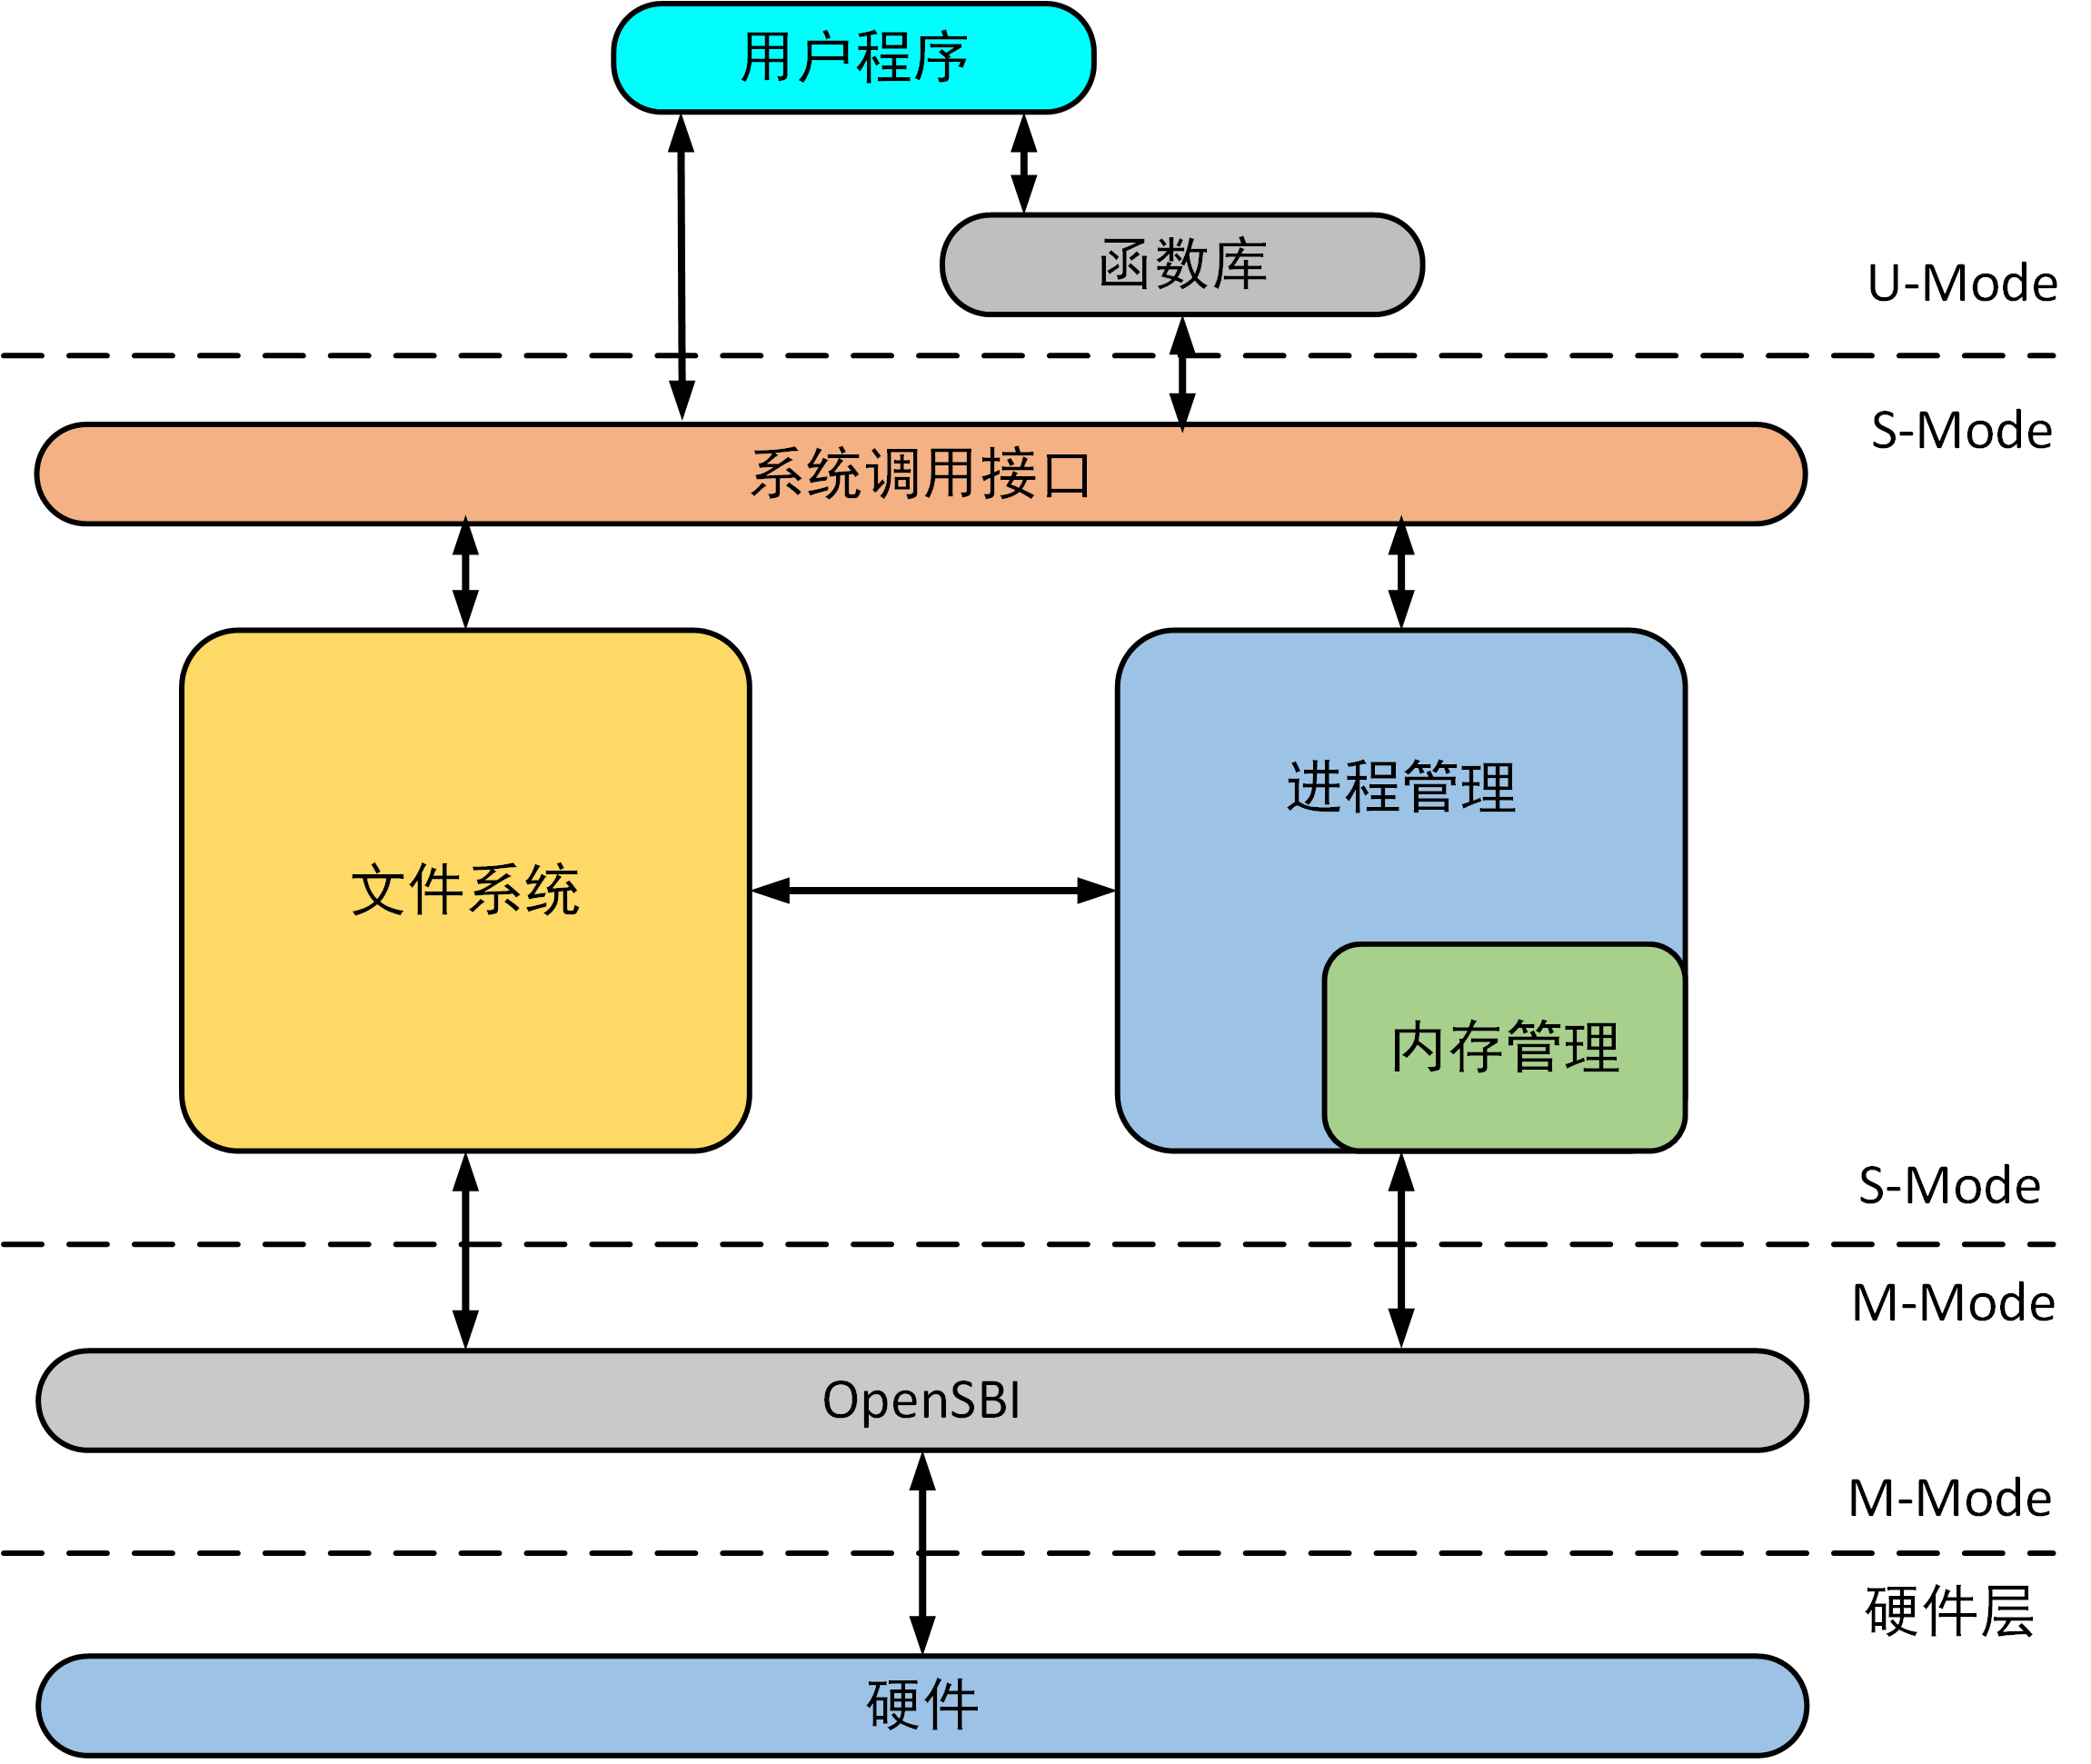
\includegraphics[width=0.55\textwidth]{moonixtotal}
	\setlength{\abovecaptionskip}{2pt}
	\caption{Moonix体系结构}
	\label{pic:moonixtotal}
\end{figure}

中断处理模块用于控制操作系统对内外部中断的响应。操作系统通过响应定时器中断,来定时检查进程的运行状态,可以说中断处理是进程调度的基础。内存管理模块主要通过虚拟内存管理的方式,保证各个进程能够安全共享物理内存,互不干扰。同时,由于各个进程都运行在独立的虚拟内存空间,使得各个程序实现时不必考虑实际的物理内存状态,降低了应用程序的实现难度。进程调度模块用来控制进程对CPU的使用,通过Round-Robin算法,来保证各个进程能够公平地使用CPU资源,同时内核也能够及时地响应外部中断。文件系统模块屏蔽了不同文件系统的细节,提供了一个通用的文件接口,供操作系统获取文件资源。
% !Mode:: "TeX:UTF-8"

\chapter{中断处理模块设计与实现}[interrupt]
\label{chapter:interrupt}

\section{模块概述}

\ref{sec:interrupt} 节中介绍过,RISC-V支持两种方式的中断处理,分别是Direct模式与Vectored模式。采用Direct模式时,当任意中断发生后,都会跳转到stvec中的BASE地址处;若是采用Vectored模式,则类似于Linux内核中使用的中断向量表,需要首先进行向量表的填充,不利于统一处理或忽略一些中断,且填表过程比较繁琐,所以Moonix中采用Direct模式来对中断进行统一处理。在中断处理函数中就可以很方便地根据中断类型来对不同的类型调用不同的处理函数分流处理流程。

在跳转进入中断处理函数之前,需要保存当前线程的CPU状态,并在退出之前恢复,以保证整个中断处理过程对线程来说是透明的。Moonix将CPU中所有的通用寄存器都保存在线程的内核栈上,并在中断函数处理结束之后将寄存器的值从内核栈上恢复到CPU,随后再跳转回原线程被中断打断的位置继续执行。

在Moonix中,中断处理需要处理以下三种最重要的中断:定时器中断、用户态(U-Mode)环境调用和外部串口中断。定时器中断主要用于线程调度,在每次定时器中断发生时,都会陷入内核并检查当前进程的剩余可执行时间,来决定是否要继续执行,更具体内容将在第 \ref{chapter:thread} 章展开说明。用户态环境调用类似于Linux中的系统调用,用于U-Mode下进程向S-Mode下操作系统请求系统功能,如输入输出、文件读写等。外部串口中断主要用于实现用户输入,因为在QEMU中,键盘被实现为一个串口设备。用户输入是一个异步事件,不可预知,为了避免需要读取键盘的线程陷入无意义的忙循环等待中,Moonix使用条件变量来实现条件等待-恢复机制,条件变量与标准输入的实现细节将在 \ref{sec:condition} 节做更深入的讨论。

\section{中断上下文的保存与恢复}

\subsection{定义中断上下文}

对于一个程序来说,某一时刻寄存器的数据和栈中的数据可以唯一确定这个程序的运行状态,由于Moonix中程序栈使用内存实现,栈顶地址保存在CPU中的sp寄存器内。因此,保存一个程序的运行状态,只需要保存这个时刻CPU中所有的通用寄存器即可。Moonix中将保存程序运行状态的数据结构成为程序上下文。

对于被中断打断的程序来说,中断处理程序应当是透明的。流程从中断处理程序恢复到原先的程序时,应当继续执行被打断的流程,并且所有的中间变量都不应当被修改,否则可能导致原先的程序发生错误。

因此,在处理中断前,Moonix需要保存所有可能被修改的寄存器,并在中断处理完成后恢复。这些包括所有的通用寄存器。同时由于scause、sepc和stval这三个寄存器,在中断发生时会被CPU自动写入中断相关信息,所以也需要额外保存。保存这三个中断信息寄存器的原因是为了使得Moonix支持中断的递归处理,即在某个中断处理的过程中,Moonix有能力保存中断处理的现场转而去处理另一个突然发生的中断。由于中断过程可能伴随特权级的变化,还需要多保存一个sstatus。

\begin{minipage}[c]{0.95\textwidth}
\begin{lstlisting}[language={C}, caption={上下文结构定义}, label={lst:context}]
typedef struct
{
	usize x[32];
	usize sstatus;
	usize sepc;
} InterruptContext;
\end{lstlisting}
\end{minipage}

Moonix中使用结构体InterruptContext来保存各种寄存器的信息,它代表的原来程序运行的上下文。InterruptContext定义如代码 \ref{lst:context} 所示。scause和stval这两个寄存器的值将在中断处理过程中作为参数传递,由于处理过程对原程序是透明的,所以无需保存这两个寄存器。

\subsection{保存中断上下文}

中断上下文需要被保存在内核栈上,由于在进入中断之前,CPU可能位于U-Mode,也可能位于S-Mode,所以需要首先判断当前模式,如果跳转之前就位于S-Mode,则无需做处理;否则需要切换sp指针到内核栈。RISC-V指令集提供了sscratch寄存器,用于保存临时栈的指针。

sscratch寄存器的使用方法可由操作系统来指定,指令集没有硬性要求,在Moonix中,若在中断之前处于U-Mode,则sscratch寄存器中保存的是内核栈地址;否则中断之前处于S-Mode,sscratch中保存的是0。这样,Moonix即可根据进入中断时的sscratch的值,来判断进入中断前的CPU状态。

\begin{minipage}[c]{0.95\textwidth}
\begin{lstlisting}[language={C}, caption={保存中断上下文}, label={lst:savecontext}]
__interrupt:
	# 交换 sscratch 和 sp
	csrrw   sp, sscratch, sp
	# 如果 sp = 0,即之前的 sscratch = 0
	# 说明是从 S-Mode 进入中断,不需要切换栈
	# 否则需要将 sp 从用户栈切换到内核栈
	# 此时的 sp 就是原来的 sscratch,就是内核栈顶地址
	# 否则还需要执行 csrr 
	bnez    sp, from_user
from_kernel:
	csrr    sp, sscratch
from_user:
	# 移动栈指针,留出 Context 的空间
	addi    sp, sp, -34*REG_SIZE
	# 保存通用寄存器,其中 x0 固定为 0
	SAVE    x1, 1
	# 循环保存 x3 至 x31 寄存器到栈上
	.set    n, 3
	.rept   29
		SAVE_N  %n
		.set    n, n + 1
	.endr
	# 若从 S-Mode 进入中断,此时 sscratch 为内核栈地址
	# 若从 U-Mode 进入中断,此时 sscratch 为用户栈地址
	# 将 sscratch 的值保存在 s0 中,并将 sscratch 清零
	csrrw   s0, sscratch, x0
	# 保存 CSR
	csrr    s1, sstatus
	csrr    s2, sepc
	# 将 sp、sstatus 和 sepc 保存到栈上 
	SAVE    s0, 2
	SAVE    s1, 32
	SAVE    s2, 33
	# 调用 handleInterrupt()
	# 将 Context 的地址(栈顶)和 scause、stval 作为参数传入
	mv      a0, sp
	csrr    a1, scause
	csrr    a2, stval
	jal     handleInterrupt
\end{lstlisting}
\end{minipage}

整个保存操作实现见代码 \ref{lst:savecontext}。中断处理的入口函数为\_\_interrupt,即stvec中的BASE字段设置为\_\_interrupt的地址。Moonix首先判断中断发生前的CPU模式,并切换到内核栈,栈指针向下移动以在栈上留出一个InterruptContext的内存区域。在保存上下文操作完成后,将sscratch的值保存在s0寄存器中,并将sscratch清零,以保证在处理中断时再次发生中断后,能满足Moonix对sscratch的规定。保存完毕后,栈上布局如图 \ref{pic:interruptframe} 所示。注意,如果进入中断前位于U-Mode,则栈上x2指向原线程的用户栈顶。

\begin{figure}[htpb]
	\centering
	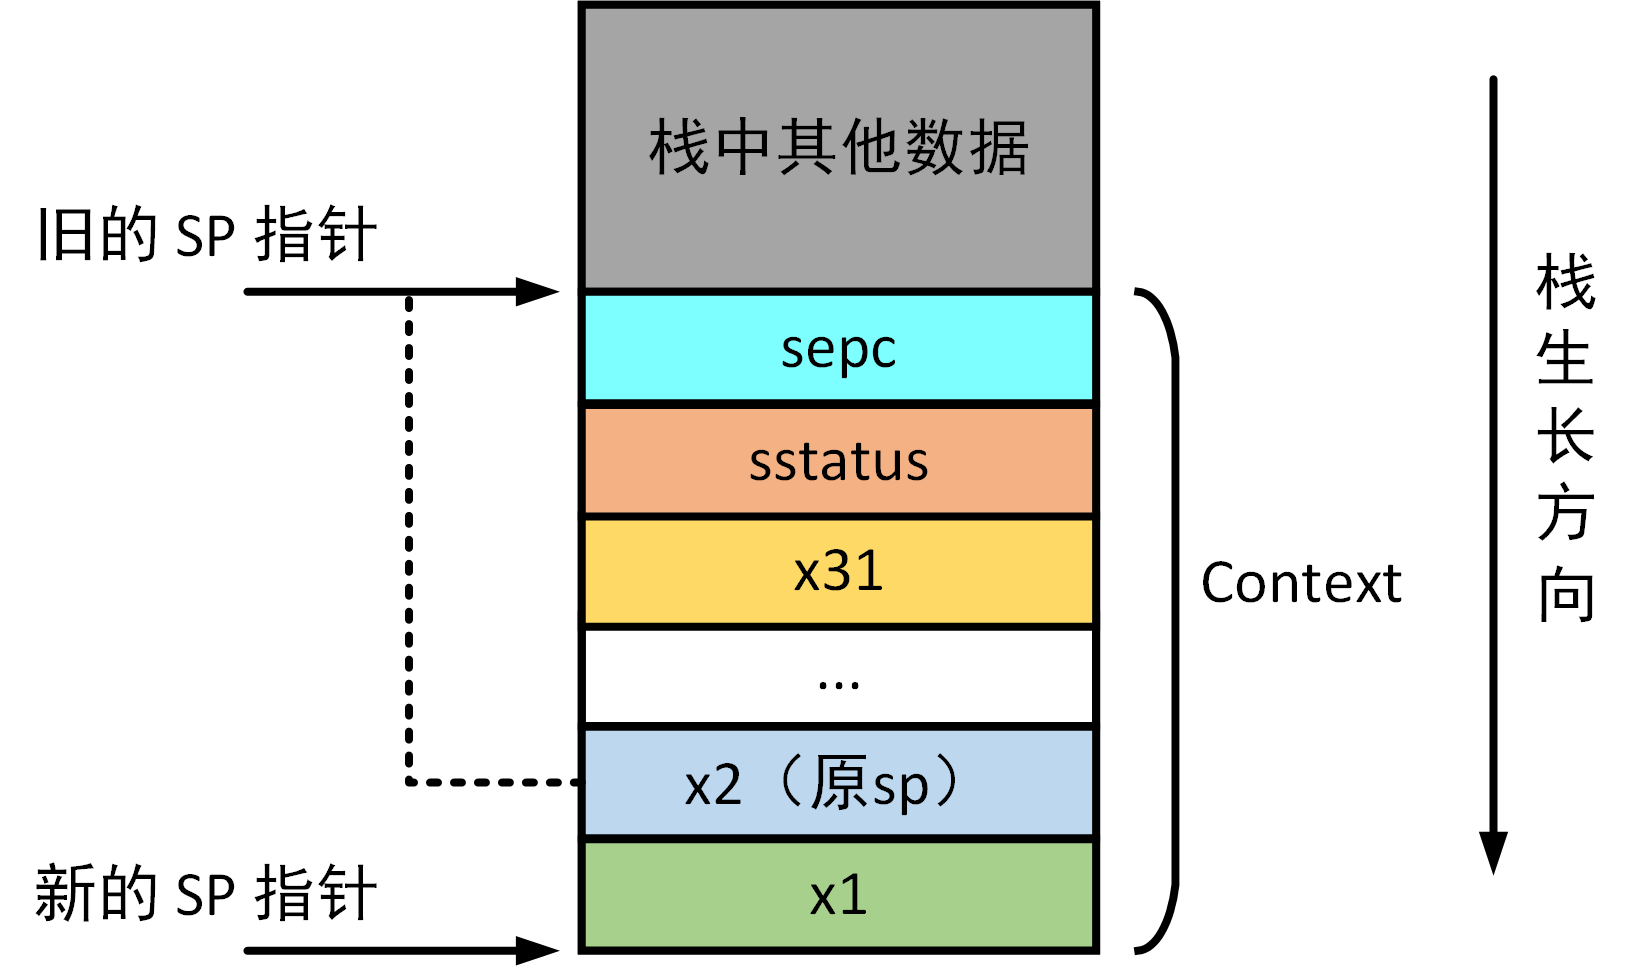
\includegraphics[width=0.7\textwidth]{interruptframe}
	\setlength{\abovecaptionskip}{2pt}
	\caption{保存中断上下文}
	\label{pic:interruptframe}
\end{figure}

完成这些操作后,Moonix就调用了handleInterrupt()函数,并将刚刚保存在内核栈上的InterruptContext地址,以及scause和stval作为参数传入函数。在handleInterrupt()函数中,就会根据scause寄存器的值来确定中断类型,并调用对应的中断处理函数来具体处理。

\subsection{恢复中断上下文}

中断处理结束后,需要从内核栈上恢复上下文,并跳转到原来中断发生时程序执行的位置。

此时sscratch已经在保存上下文时清零了。如果中断发生前CPU处于U-Mode,Moonix需要在返回前将sscratch置为内核栈顶的地址,内核栈顶地址已经保存在寄存器s0中,只需要减去InterruptContext占据的空间即可。

由于此时sscratch已经无法用于判断中断前模式,恢复时借助sstatus寄存器的SPP位。整个恢复过程如代码 \ref{lst:restorecontext} 所示。

Moonix最后执行sret指令,控制流将跳转到sepc寄存器中保存的地址处,即中断发生的位置。同时,CPU会被设置为sstatus中的SPP位标记的模式,由于中断处理过程中没有对sstatus寄存器做过修改,所以会切换会进入中断前的模式。

在Moonix线程创建时,将借助中断恢复的机制来对线程的模式和寄存器等进行设置填充,以进行初始化。更具体的细节见第 \ref{chapter:thread} 章。


\begin{minipage}[c]{0.95\textwidth}
\begin{lstlisting}[language={C}, caption={恢复中断上下文}, label={lst:restorecontext}]
__restore:
	# 恢复 CSR
	LOAD    s1, 32
	LOAD    s2, 33
	# 如果从 S-Mode 进入中断, sstatus 的 SPP 位为 1
	# 如果从 U-Mode 进入中断, sstatus 的 SPP 位为 0
	andi    s0, s1, 1 << 8
	bnez    s0, to_kernel
to_user:
	# 释放内核栈空间
	addi    s0, sp, 34 * REG_SIZE
	# 如果从 U-Mode 进入中断
	# 则此时 sscratch 指向用户栈顶
	# 令其指向内核栈顶地址
	csrw    sscratch, s0
to_kernel:
	# 恢复 sstatus 和 sepc
	csrw    sstatus, s1
	csrw    sepc, s2
	# 恢复通用寄存器
	LOAD    x1, 1
	# 恢复 x3 至 x31
	.set    n, 3
	.rept   29
		LOAD_N  %n
		.set    n, n + 1
	.endr
	# 最后恢复 sp(这里最后恢复是为了上面可以正常使用 LOAD 宏)
	LOAD    x2, 2
	sret
\end{lstlisting}
\end{minipage}

\section{条件变量与标准输入缓冲的实现}
\label{sec:condition}

条件变量在Moonix中,主要用于实现标准输入缓冲。条件变量和标准输入缓冲主要基于这样的场景提出的:一个用户进程通过getc()函数发起了一个系统调用,用于获取一个键盘输入的字符,内核处理调用的时候发现,当前并没有字符输入。这时,一个很简单的想法就是进入一个忙循环,不断地检查是否有字符输入,直到有字符输入后再将其读出,系统调用返回。这种方式肯定能保证读到字符,但是线程会占用资源,什么都不做,浪费CPU资源,即使会被CPU调度,但是所有属于该线程的时间片都被浪费掉了。

Moonix使用条件变量机制来解决这个问题,当线程检查到当前没有键盘输入时,就自动进入睡眠状态,同时不再参与调度,直到有字符输入时,才会将这个线程唤醒参与调度,这个时候被唤醒的线程就一定可以获取到字符并返回了。这样这个问题就被转化成了一个典型的生产者消费者问题。

标准输入缓冲维护了一个字符队列和一个条件变量,而条件变量也只是维护了一个等待队列,保存了等待条件满足的线程的tid。Moonix定义结构如代码 \ref{lst:stdin} 所示。

\begin{minipage}[c]{0.95\textwidth}
\begin{lstlisting}[language={C}, caption={标准输入缓冲和条件变量}, label={lst:stdin}]
typedef struct {
	Queue waitQueue;
} Condvar;

struct
{
	Queue buf;
	Condvar pushed;
} STDIN;
\end{lstlisting}
\end{minipage}

当一个线程排队进入临界区尝试获取输入的字符时,如果字符队列中有字符,则直接获取返回。若无字符,则将自身放入等待队列中并挂起。当有字符被输入时,Moonix会首先将字符存入字符队列,并检查等待队列中是否有线程在等待,如果有则唤醒队首线程,该线程会重新尝试进入临界区获取字符。整个流程示意如图 \ref{pic:stdin}。

\begin{figure}[htpb]
	\centering
	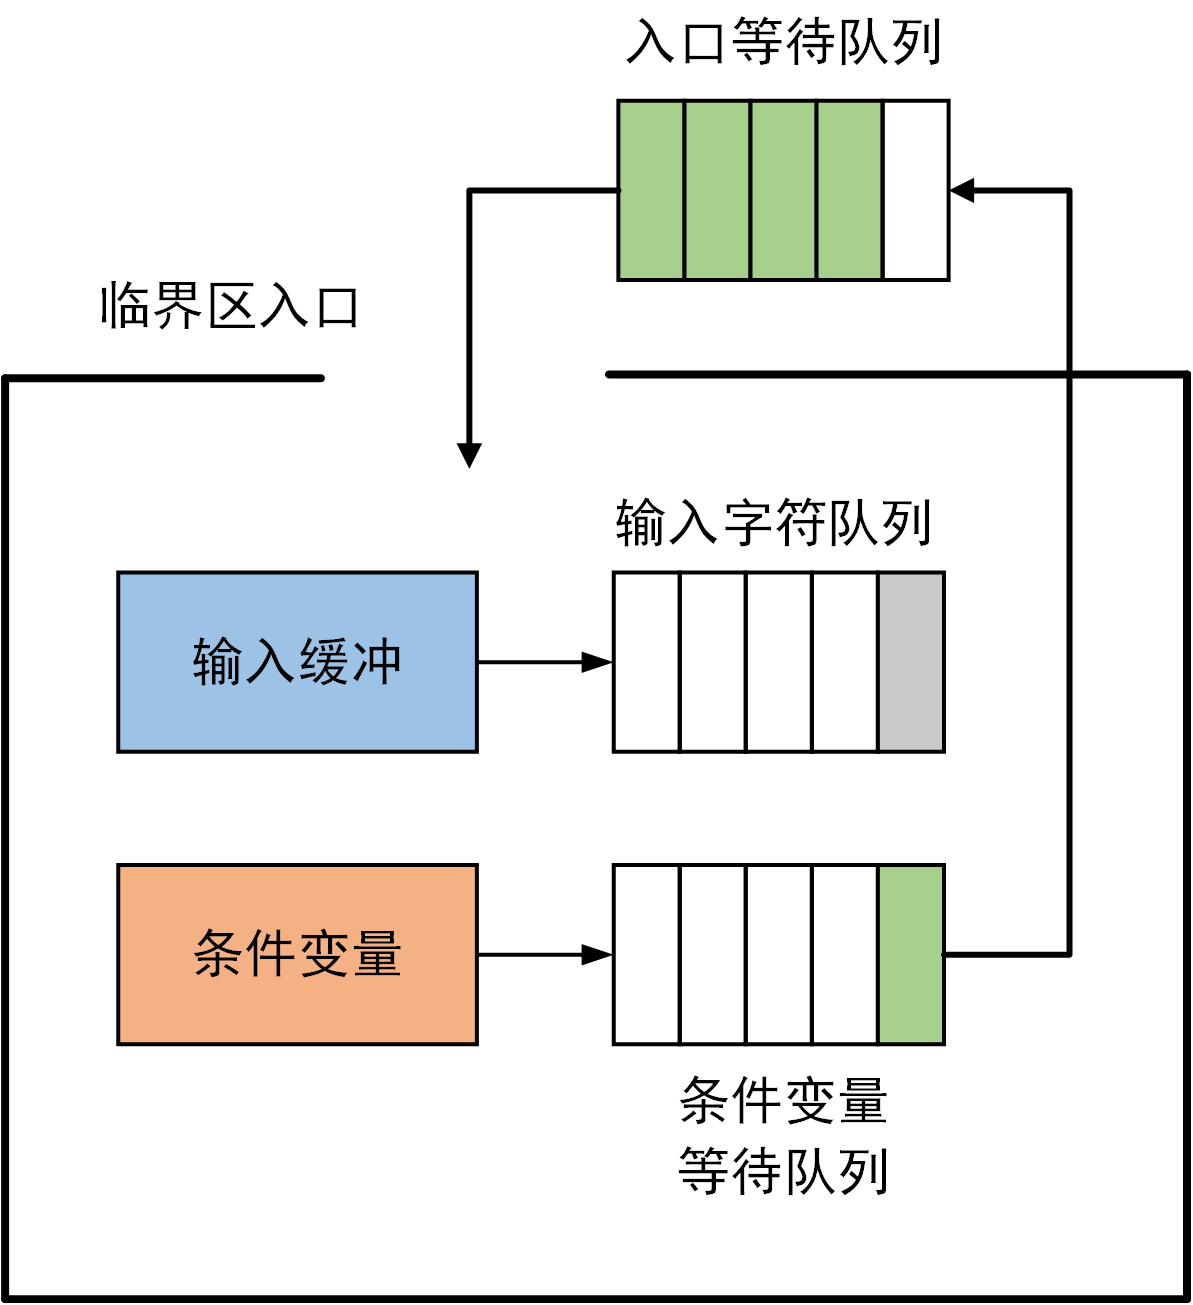
\includegraphics[width=0.5\textwidth]{stdin}
	\setlength{\abovecaptionskip}{2pt}
	\caption{标准输入缓冲区示意}
	\label{pic:stdin}
\end{figure}
% !Mode:: "TeX:UTF-8"

\chapter{内存管理模块设计与实现}[memory]
\label{chapter:memory}

\section{模块概述}

Moonix采用两种粒度来对可用的内存进行管理。一种是动态内存分配,另一种是按页进行的内存分配。动态内存分配用于在运行时程序主动请求少量内存的情况。对Moonix来说,动态内存分配的目标是BSS段中一个8 MB大的内存空间;对于应用程序来说,应用程序运行环境也为每个进程都提供了一片内存空间用于动态内存分配。Moonix采用Buddy System Allocation算法来对堆空间进行管理,并按照最小64字节的粒度对堆空间进行划分分配。按页内存分配的分配主体是除去内核以外的所有空闲物理内存,Moonix使用一棵线段树来维护这段内存空间的使用情况。这两种分配都采用外挂式数据结构实现,以降低侵入性和代码耦合度。Moonix同样需要借助按页内存分配来实现物理内存映射到虚拟内存空间。

Moonix采用Rv64架构提供的Sv39系统来实现虚拟内存。在操作系统初始化时,Moonix就会将内核映射到虚拟地址空间,并在创建用户进程的时候都会创建独立的虚拟地址空间,即创建不同的页表来表示不同的映射模式。这样可以将不同进程的代码和数据隔离,在切换到进程时,需要切换到对应进程的页表,这部分将在第 \ref{chapter:thread} 章具体描述。

\section{动态内存分配}

\subsection{Buddy System Allocation算法概述}

动态内存分配是在程序运行过程中,程序动态请求内存空间,操作系统响应而进行的内存分配。通常,操作系统会为每个进程分配一块堆内存空间,该进程执行过程中的动态内存分配都在这块内存上进行。那么该使用怎么的策略进行内存分配就成了操作系统亟待解决的问题。

一个很简单的想法就是,我们可以不断地分配最小的可用地址,这样一直分配下去,内存看起来都是连续的。
但是,在此过程中,如果中间有一块内存被回收了,那么这块内存即使是可用的,但是由于其两边都是被占用的内存,这块空闲区间已经无法被扩展,最终形成外部碎片。
随着不断回收和分配内存,整块内存区间可能产生越来越多的外部碎片,以至于某个时刻,我们可能需要分配一块较大的内存,几个外部碎片的空间之和是足够的,但是单个外部碎片是无法满足需要的。这时可能会想到JVM中的标记整理算法,通过将所有可用的内存向一边移动,来减少外部碎片,这种方式的开销较大,因为操作系统不得不同步更改所有代码或数据中的地址。

Buddy System Allocation是一种经典的内存分配算法\cite{DBLP:journals/acta/BrodalDM05},被大量操作系统实现使用,包括Linux。Buddy System将整块内存按2的幂划分成若干小块,并搜索由小块形成的空闲链表并给出所需求的最佳匹配的大小。该算法的优点可以以较小的时间复杂度(O(logN))快速寻找到合适的空闲块,同时可以快速合并两个相邻的同大小空闲块。同时,由于采用最佳适配的策略,使用该算法进行内存分配会产生较少的外部碎片。该算法的缺点是会产生内部碎片,例如如果要分配66个单位,那么必须划分128单位的块,内部多出来的内存空间就无法被使用了。

\subsection{动态内存分配实现}

在Moonix中,内核的动态内存分配主体,是bss段的一块8 MB大小的内存区域。Moonix将最小划分的块定为64字节,这个大小是基于空间上的考虑,将在本节最后给出这种方案的内存开销。

Moonix使用一棵二叉树来存储每一级范围内的最大连续空闲块个数。最底层的节点代表每个最基本的64字节内存块的使用情况,第二层的每一个节点则代表两个64字节内存块,即一个128字节范围的使用情况。以此类推,最顶层的单个节点就表示全部的8 MB大小的内存区域的使用情况。如图 \ref{pic:buddysystem} 所示。

\begin{figure}[htpb]
	\centering
	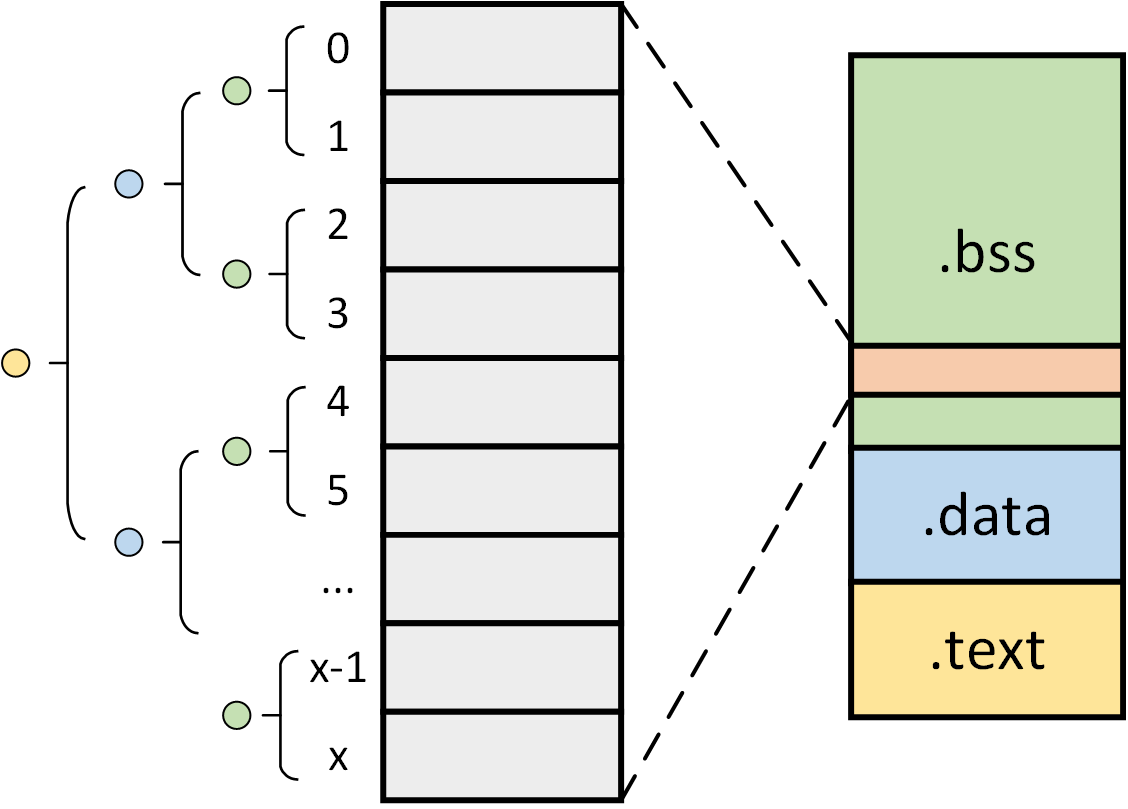
\includegraphics[width=0.65\textwidth]{buddysystem}
	\setlength{\abovecaptionskip}{2pt}
	\caption{保存中断上下文}
	\label{pic:buddysystem}
\end{figure}


\begin{minipage}[c]{0.95\textwidth}
\begin{lstlisting}[language={C}, caption={动态内存分配管理二叉树}, label={lst:mallocbinary}]
struct
{
	int size;
	int longest[BUDDY_NODE_NUM];
} buddyTree;
\end{lstlisting}
\end{minipage}

二叉树的每个节点的值表示该节点所代表的范围内最多可以使用的连续空闲块的个数,这个数值是由该节点下层每一级的节点数值取较大值得出的,原理类似于胜者树的调整过程。Moonix中定义的用于管理动态内存分配的二叉树结构如代码 \ref{lst:mallocbinary} 所示。size域为整棵二叉树管理的总内存块的个数,而longest数值记录了二叉树每个节点的值。其中,BUDDY\_NODE\_NUM的值应当等于$size<<2-1$。\\

\begin{algorithm}[H]
	\SetKwInOut{KIN}{\textbf{输入}}
	\SetKwInOut{KOUT}{\textbf{输出}}
	\KIN{待分配的内存块个数}
	\KOUT{分配的内存区域的首块块号}
	
	设置所需内存块个数为大于等于输入数量的最小的2的幂\;
	设置当前节点为二叉树根节点\;
	\While{当前节点大小 != 所需内存块个数}{
		\eIf{左分支节点较小且满足条件}{
			将左分支节点设置为当前节点\;
		}{
			将右分支节点设置为当前节点\;
		}
	}
	将当前节点的值设为0\;
	将临时节点设置为当前节点\;
	\While{临时节点 != 根节点-1}{
		将当前临时节点的父节点设置为临时节点\;
		将当前临时节点的值设置为左右分支的最大值\;
	}
	返回当前节点对应范围的第一个块号\;
	\caption{动态内存分配}
	\label{alg:kalloc}
\end{algorithm}

\vspace{12 pt}

分配过程对应于算法 \ref{alg:kalloc}。其中算法第四行中优先寻找较小的且满足条件的块,这样分配会尽量保留大块,减小外部碎片。该算法的另一个实现可能会寻找第一个满足条件的块,这样会产生较多的外部碎片而导致分配效率降低。

注意在分配时,只会标记被分配节点的使用情况,而不会修改其下级节点的值,这样是为了在回收时可以快速确定最初被分配出去的节点。

在通过分配算法标记二叉树中的占用情况,并返回第一个块的块号后,即可根据块号和块的大小,计算出相对于堆空间起始地址的偏移,最终得到这块可用内存的地址。

下面来计算使用Buddy System Allocation算法管理堆内存时所需要的额外内存开销。

如果我们想要管理8 MB,即$2^{23} Byte$的内存,最小分配的块大小是$64 Byte = 2^6 Byte$,那么要管理的内存空间可划分为$2^{17}$块,用于管理的满二叉树共有$2^{18} - 1$个节点,每个节点是一个四字节的无符号整数,BuddyTree所占用的内存空间$2^{20} Byte$,即1 MB。Moonix只需要额外花费1 MB内存,就可以管理这8 MB的堆内存空间。

\section{按页内存分配}

按页内存分配的主体是整个可用的物理内存,首先需要确定可用的物理内存范围。Moonix目前运行在QEMU虚拟机模拟的Virt机器上,Virt机器将128MB的物理内存安排在0x80000000到0x88000000空间上。这块可用的内存空间就是按页内存分配的主体。

Moonix使用一棵非递归线段树来对这块内存进行管理。事实上,非递归版本的线段树和第一节提到的Buddy System Allocation算法的结构非常类似,同样也是一棵二叉树管理2的幂级数长度的区间。唯一不同的是,按页内存分配不需要记录该区间上还有多少空闲页,因为一次只分配一页。这样,每个节点只需要记录一个布尔类型的值,即该区间上是否有空闲页。

由于思想基本一致,不再赘述其思想与实现。

\section{虚拟地址空间}

Moonix使用Sv39系统来实现虚拟地址空间,以实现进程间代码数据隔离与共享,并固定进程的内存布局,降低应用程序编写的难度。同时,通过页表还可以提供对特定内存区域的访问控制,以防止恶意应用程序任意读写执行内存。

\begin{minipage}[c]{0.95\textwidth}
\begin{lstlisting}[language={C}, caption={页表相关数据结构定义}, label={lst:pagetable}]
typedef usize PageTableEntry;   /* 页表项长度 64 位 */
/*
* 页表由页表项组成 
* 一页页表中包含 4096 / 8 个页表项
*/
typedef struct
{
	PageTableEntry entries[PAGE_SIZE >> 3];
} PageTable;
\end{lstlisting}
\end{minipage}

Moonix将内核区域分成如表 \ref{tab:sectionprivilege} 所示的几个部分,并分别定义了是否可读可写可执行的访问权限。

\begin{table}[h]
	\centering
	\caption{Moonix中各个段权限}
	\label{tab:sectionprivilege}
	\begin{tabular}{|c|c|c|c|}
		\hline
		段名      & 可读 & 可写 & 可执行 \\ \hline
		.text   & 是  & 否  & 是   \\ \hline
		.rodata & 是  & 否  & 否   \\ \hline
		.data   & 是  & 是  & 否   \\ \hline
		.bss    & 是  & 是  & 否   \\ \hline
		剩余空间    & 是  & 是  & 否   \\ \hline
	\end{tabular}
\end{table}

Moonix中,为了方便操作页表和页表项相关的数据结构,将相关结构定义如代码 \ref{lst:pagetable}。

虚拟内存映射的难点在于,如何递归创建页表结构并填充。Moonix采用一个比较巧妙的方式,在查找页项的同时,如果发现对应层级的页表还没有构造,就动态申请一块内存用作页表,并记录在上层页表项中。这样在映射的过程中,就只会创建使用到的内存区域对应的下级页表,而无需构建全部的页表了。查找页表项并构建所需的下级页表的实现见代码 \ref{lst:createpagetable}。

在完成页表项和页表的构建之后,只需要将根页表的物理页号写入satp寄存器中,CPU就会在取得虚拟地址时,自动地进行地址翻译。

同样,当用户进程执行时,除了要将内核映射到用户进程的高地址处以外,还需要将进程自己的代码和数据映射到虚拟地址空间的低地址位,同时,还需要设置进程的代码和数据的页表项的U标志位,以保证该内存区域可以在U-Mode下访问。

\begin{minipage}[c]{0.95\textwidth}
\begin{lstlisting}[language={C}, caption={查找页表项}, label={lst:createpagetable}]
	PageTableEntry
	*findEntry(Mapping self, usize vpn)
	{
		PageTable *rootTable = (PageTable *)accessVaViaPa(self.rootPpn << 12);
		usize *levels = getVpnLevels(vpn);
		PageTableEntry *entry = &(rootTable->entries[levels[0]]);
		int i;
		for(i = 1; i <= 2; i ++) {
			if(*entry == 0) {
				// 页表不存在,创建新页表
				usize newPpn = allocFrame() >> 12;
				*entry = (newPpn << 10) | VALID;
			}
			usize nextPageAddr = (*entry & PDE_MASK) << 2;
			entry = &(((PageTable *)accessVaViaPa(nextPageAddr))->entries[levels[i]]);
		}
		return entry;
	}
\end{lstlisting}
\end{minipage}
% !Mode:: "TeX:UTF-8"

\chapter{线程调度模块设计与实现}[thread]
\label{chapter:thread}

\section{模块概述}

进程是一个处于运行状态的程序实例,拥有自己的内存空间和运行时数据。Moonix采用了一个最简单的进程模型:进程和线程一一对应,即一个进程中只包含一个线程。这样,CPU实际上只是在调度线程,进程剥离出线程之后,就只剩下资源分配的属性了。Moonix中,一个进程保有一个页表和一个文件描述符数组:页表代表这个进程的独立的虚拟地址空间,文件描述符则表示这个进程打开的文件。

当一个线程运行时,能代表一个线程的运行状态的切面数据,称为这个线程的上下文。这个切面由CPU中所有的寄存器和栈中的数据组成。理论上,只要恢复线程上下文,就可以恢复线程保存上下文时的状态。和中断类似,在线程切换时,需要将上一个线程的上下文保存起来,以便在未来某个时刻重新切换回这个线程时,能够继续之前的状态运行下去。内核中线程的数据结构中保存了该线程的上下文地址,由于上下文总是存放在线程栈顶,所以该地址也是栈顶地址。

线程调度依赖于时钟中断。当时钟中断发生时,内核采用round robin算法\cite{DBLP:journals/eor/RasmussenT08},检查当前线程的时间片,并决定是否将暂停当前线程的运行,而将CPU资源让出。

Moonix中线程状态由线程池维护,线程的状态分为四种,分别如下:

\begin{itemize}
	\item 就绪状态(Ready):线程处于就绪队列中,等待被 CPU 调度执行
	\item 运行状态(Running):线程此时正占有 CPU 运行
	\item 睡眠状态(Sleeping):线程等待某个条件满足,此时线程不会被调度执行,直到条件满足后才会被加入就绪队列
	\item 退出状态(Exited):线程已经完成了任务执行,但是还没有回收资源
\end{itemize}

状态之间的切换及条件如图 \ref{pic:threadstatus} 所示。

\begin{figure}[htpb]
	\centering
	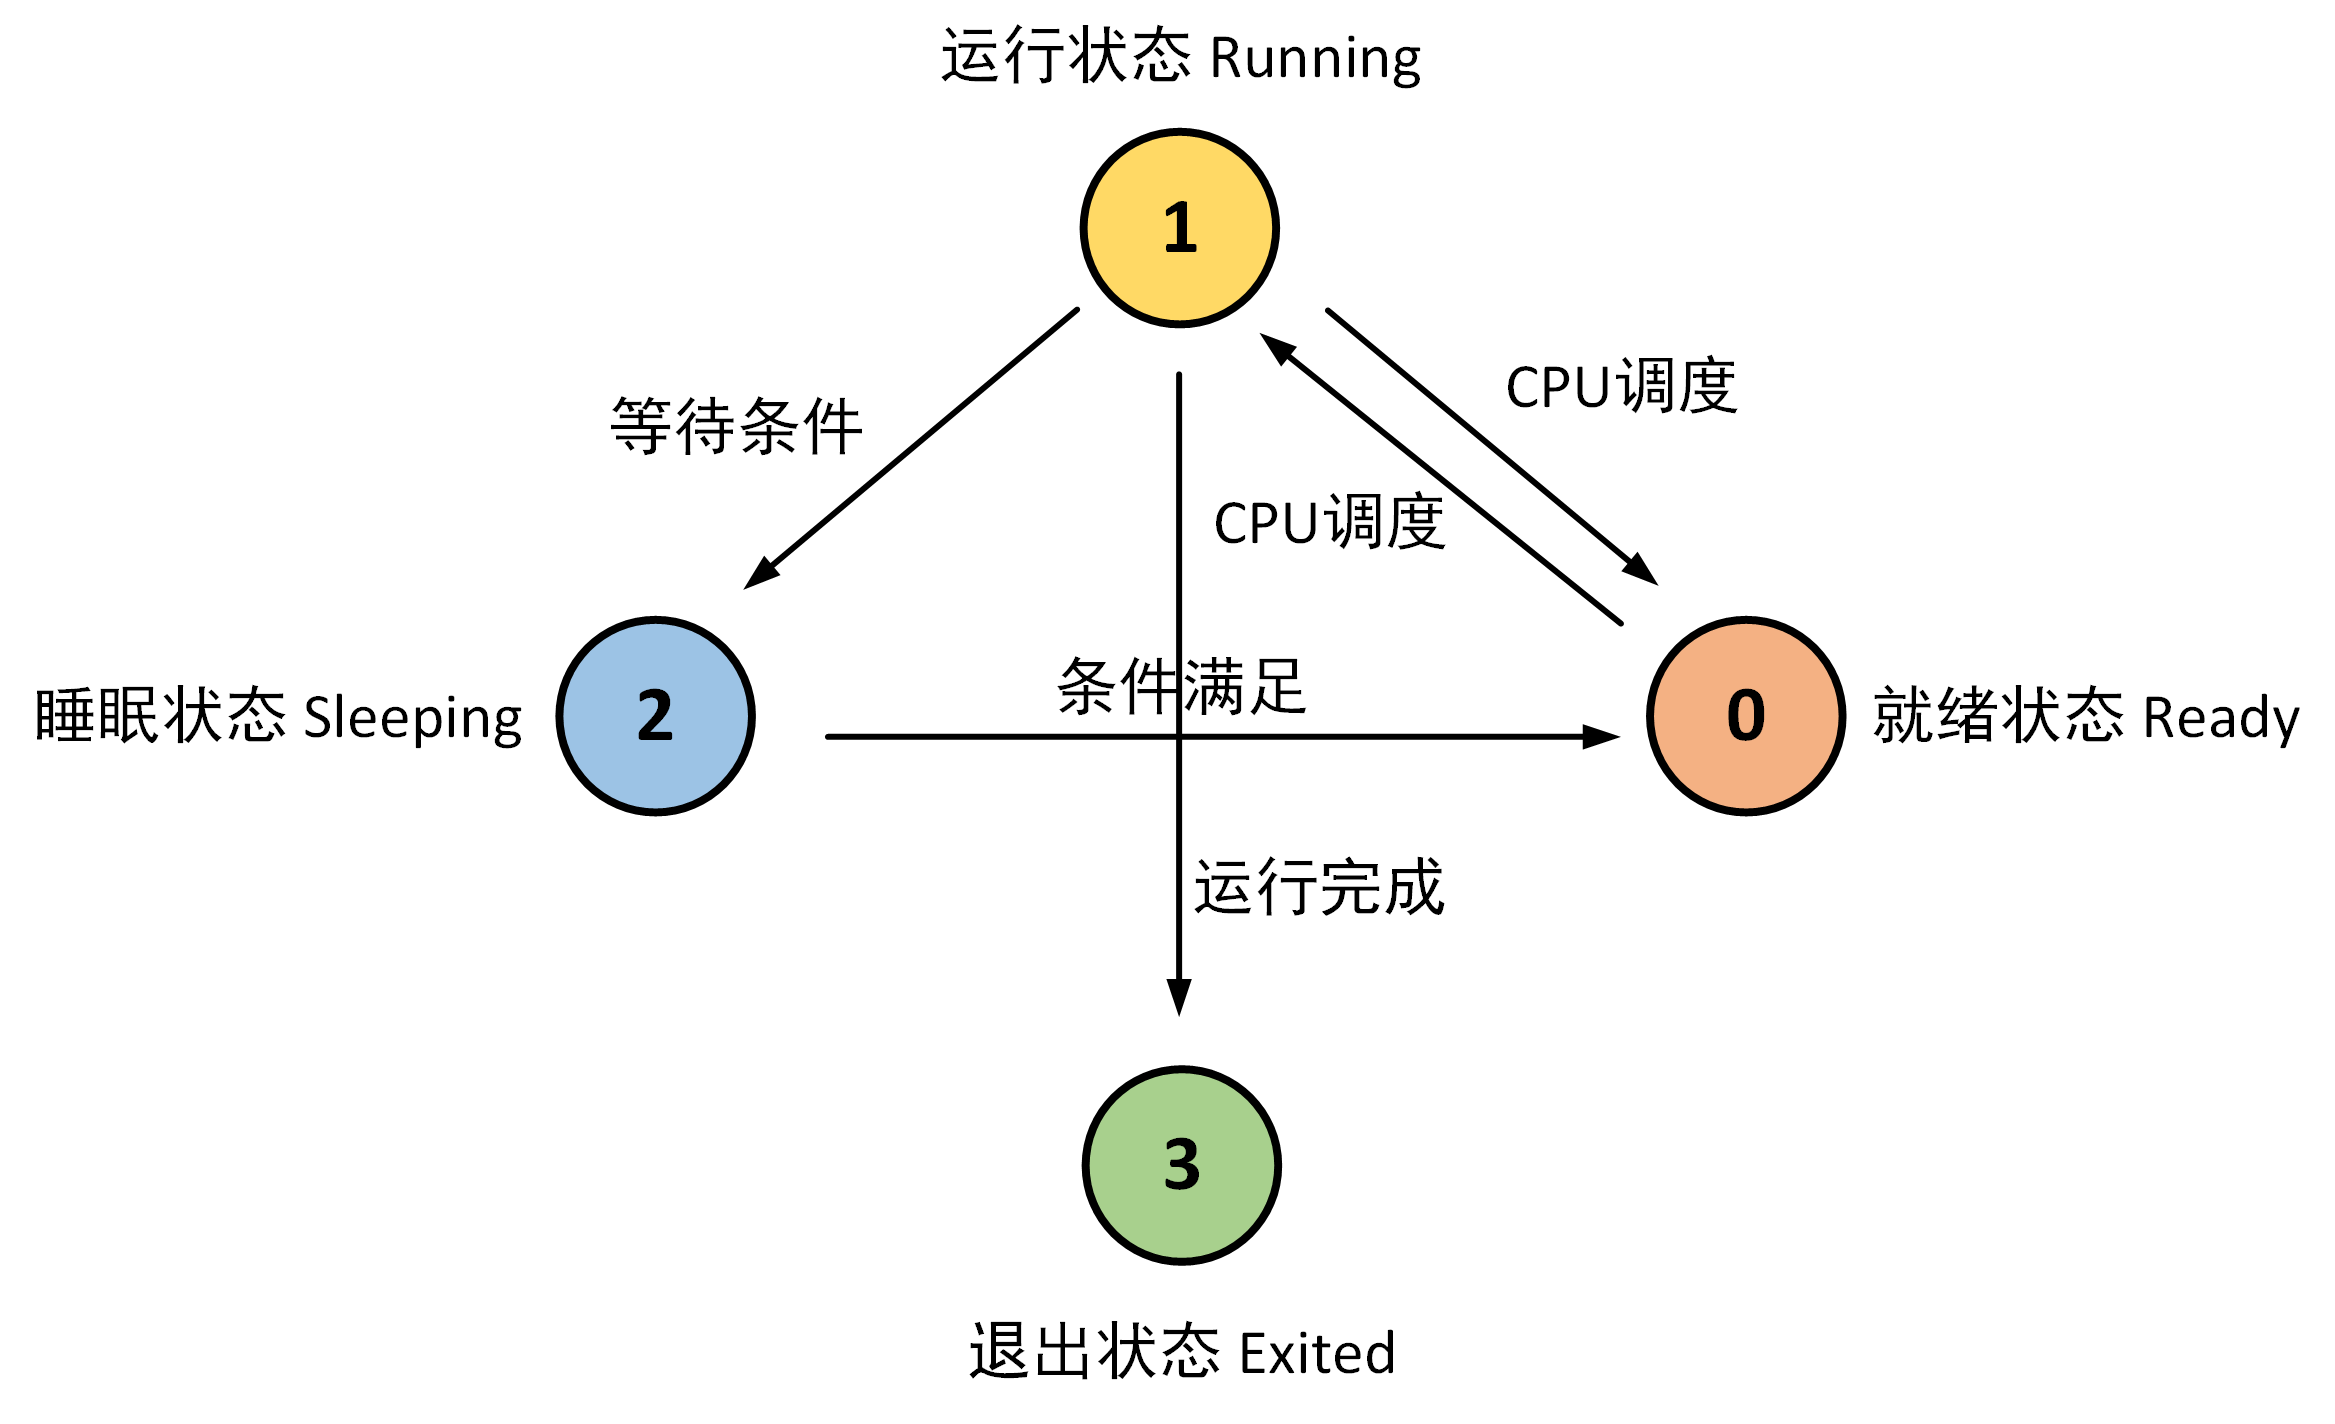
\includegraphics[width=0.7\textwidth]{threadstatus}
	\setlength{\abovecaptionskip}{2pt}
	\caption{保存中断上下文}
	\label{pic:threadstatus}
\end{figure}

\section{线程的启动和切换}

Moonix中将线程结构定义为如代码 \ref{lst:threadstructure} 的结构体。而实际上,在执行中,并不会用到kstack域,启动和切换基本只涉及contextAddr域。

\begin{minipage}[c]{0.95\textwidth}
\begin{lstlisting}[language={C}, caption={线程结构定义}, label={lst:threadstructure}]
typedef struct {
	usize contextAddr;  /* 线程上下文存储的地址 */
	usize kstack;       /* 线程栈底地址 */
} Thread;
\end{lstlisting}
\end{minipage}

类似于中断上下文保存,Moonix也可以将全部的寄存器作为上下文直接保存在栈上。实际实现中,Moonix将线程上下文切换的汇编内联到一个C函数switchContext中,通过调用该函数来进行上下文的切换。根据函数调用规范,在流程进入线程切换的函数时,就会自动保存调用者保存的寄存器到栈上。而在后续在切换回到该线程后,会首先从函数中返回,这部分寄存器的值会自动从栈上被恢复。函数调用规范由编译器负责实现,Moonix无需手动进行保存。采用这种方式进行切换线程上下文,就无需像中断一样保存全部的通用寄存器了。事实上,Moonix只需要手动保存以下的内容:

\begin{itemize}
	\item ra 寄存器,用于保存返回地址
	\item satp 寄存器,保存页表信息,本章的线程都可以说是同属于内核进程的,共用一个页表
	\item s0 \textasciitilde s11,函数调用中被调用者保存的寄存器
\end{itemize}

\begin{minipage}[c]{0.95\textwidth}
\begin{lstlisting}[language={C}, caption={线程上下文定义}, label={lst:threadcontext}]
typedef struct {
	usize ra;
	usize satp;
	usize s[12];
} ThreadContext;
\end{lstlisting}
\end{minipage}

于是定义线程上下文如代码 \ref{lst:threadcontext}。

Moonix在启动后,实际上是位于一个启动线程中的。Moonix需要构造一个“静止”的线程,一个静止线程的结构看起来就像是刚刚被CPU抢断后保存的结构。这样,当其他正在运行的线程切换到它时,就可以将寄存器和栈变成预期的初始化状态,并且跳转到程序的入口开始运行。

Moonix在创建新线程时,会统一将线程的入口ra设置为\_\_interrupt函数,并创建一个InterruptContext,填充其中的寄存器的值。而线程的真正入口,则保存在InterruptContext中的sepc域中。同时,申请一段内存作为新线程的线程栈,将InterruptContext和ThreadContext分别压入栈底,新线程的线程栈顶,就是ThreadContext结构。

在切换进新线程时,会首先将栈指针切换为新线程的线程栈顶,切换上下文的逻辑会将栈顶的ThreadContext中的内容恢复到CPU中,并执行ret指令跳转到ra寄存器中保存的地址处。这个跳转不会涉及特权模式的变化,跳转之后仍然处于S-Mode。在创建线程时,ra被统一写为\_\_interrupt函数的地址,此时栈顶收缩至ThreadContext下方的InterruptContext处。

Moonix中断恢复的代码 \ref{lst:restorecontext} 逻辑中,中断恢复时会自动将栈顶的InterruptContext中的内容都恢复到寄存器中,并执行sret跳转到sepc寄存器中保存的地址处。此时InterruptContext恰好位于栈顶。接下来的事情就顺理成章了:中断恢复函数会将InterruptContext中的内容全部恢复到CPU中,包括传入的参数和sepc,随后sret指令将流程跳转到sepc寄存器保存的地址处,即最初设置的线程的真正的入口处。sret指令还可以修改CPU的运行模式,可以通过修改sstatus寄存器的SPP位,来实现不同的运行模式下的线程。

\section{线程池与线程管理}

Moonix中,调度器scheduler只是对线程的id进行调度管理,和实际的线程结构没有直接关系。因此,Moonix使用线程池ThreadPool结构,来给Tid和线程结构建立联系,将调度器对线程Tid的调度转换成线程池对实际线程的调度。线程池的定义如代码 \ref{lst:threadpool} 所示。

通过线程池,线程的调度会被线程池中的Scheduler代理实现,从Scheduler中获取到线程id后,再由线程池在threads数组中操作真正的线程结构。当一个新线程被创建时,也需要由线程池分配一个可用的线程id。

\begin{minipage}[c]{0.95\textwidth}
\begin{lstlisting}[language={C}, caption={线程池定义}, label={lst:threadpool}]
	/* 线程池中的线程信息槽 */
	typedef struct {
		Status status;
		int tid;
		int occupied;       /* 该槽位是否被占用 */
		Thread thread;
	} ThreadInfo;
	
	typedef struct {
		ThreadInfo threads[MAX_THREAD];
		Scheduler scheduler;
	} ThreadPool;
\end{lstlisting}
\end{minipage}

\section{线程调度}

Moonix线程调度依赖于时钟中断,时钟中断的中断处理函数除去预约下一次时钟中断外,还会额外去进行线程调度的工作。

Moonix所有的运行流程都是运行在线程中的,由于要对所有的线程进行调度,Moonix创建了一个调度线程,专用于线程的切换与调度。Moonix中,这个线程被命名为Idle线程。具体来说,Idle线程的作用是:

\begin{enumerate}
	\item 当没有线程在运行时,调度线程根据一定的策略来选择一个线程来执行
	\item 当一个线程被调度器判断需要让出 CPU 控制权时,例如运行时间过长或者运行结束,并不是直接切换到另一个线程,而是先切换到这个调度线程,让调度线程根据一定的策略来选择另一个线程执行
\end{enumerate}

Moonix中定义了一个结构体Processor,用来保存调度线程参与调度所需要的所有信息,如代码 \ref{lst:processor}。其中idle字段就是调度线程,current字段描述了当前正在运行线程的信息,occupied字段表示当前是否有线程(除了调度线程)正在运行。Idle线程所有的调度都是直接依赖Processor结构进行的。

\begin{minipage}[c]{0.95\textwidth}
\begin{lstlisting}[language={C}, caption={Processor结构体}, label={lst:processor}]
typedef struct {
	ThreadPool pool;
	Thread idle;
	RunningThread current;
	int occupied;
} Processor;
\end{lstlisting}
\end{minipage}

Idle线程的入口点即为idleMain函数,如代码 \ref{lst:idlemain} 所示。

\begin{minipage}[c]{0.95\textwidth}
\begin{lstlisting}[language={C}, caption={idleMain函数}, label={lst:idlemain}]
void
idleMain()
{
	// 进入 idle 时禁用异步中断
	disable_and_store();
	while(1) {
		RunningThread rt = acquireFromPool(&CPU.pool);
		if(rt.tid != -1) {
			// 有线程可以运行
			CPU.current = rt;
			CPU.occupied = 1;
			printf("\n>>>> will switch_to thread %d in idle_main!\n", CPU.current.tid);
			switchThread(&CPU.idle, &CPU.current.thread);
			
			// 切换回 idle 线程处
			printf("<<<< switch_back to idle in idle_main!\n");
			CPU.occupied = 0;
			retrieveToPool(&CPU.pool, CPU.current);
		} else {
			enable_and_wfi();
			disable_and_store();
		}
	}
}
\end{lstlisting}
\end{minipage}

idleMain函数首先关闭中断响应,以防止调度过程被中断打断,造成混乱。接着尝试从线程池中获取一个可执行的线程,切换到该线程开始执行。当某个时刻时间片用完后,内核会切换回idle线程,流程会返回idleMain的第16行,并进入下一次循环。如果没有线程可供执行,idle线程会打开中断。

从一个正在运行的线程的角度来说,整个流程时间线如图 \ref{pic:threadswitch} 所示。

\begin{figure}[htpb]
	\centering
	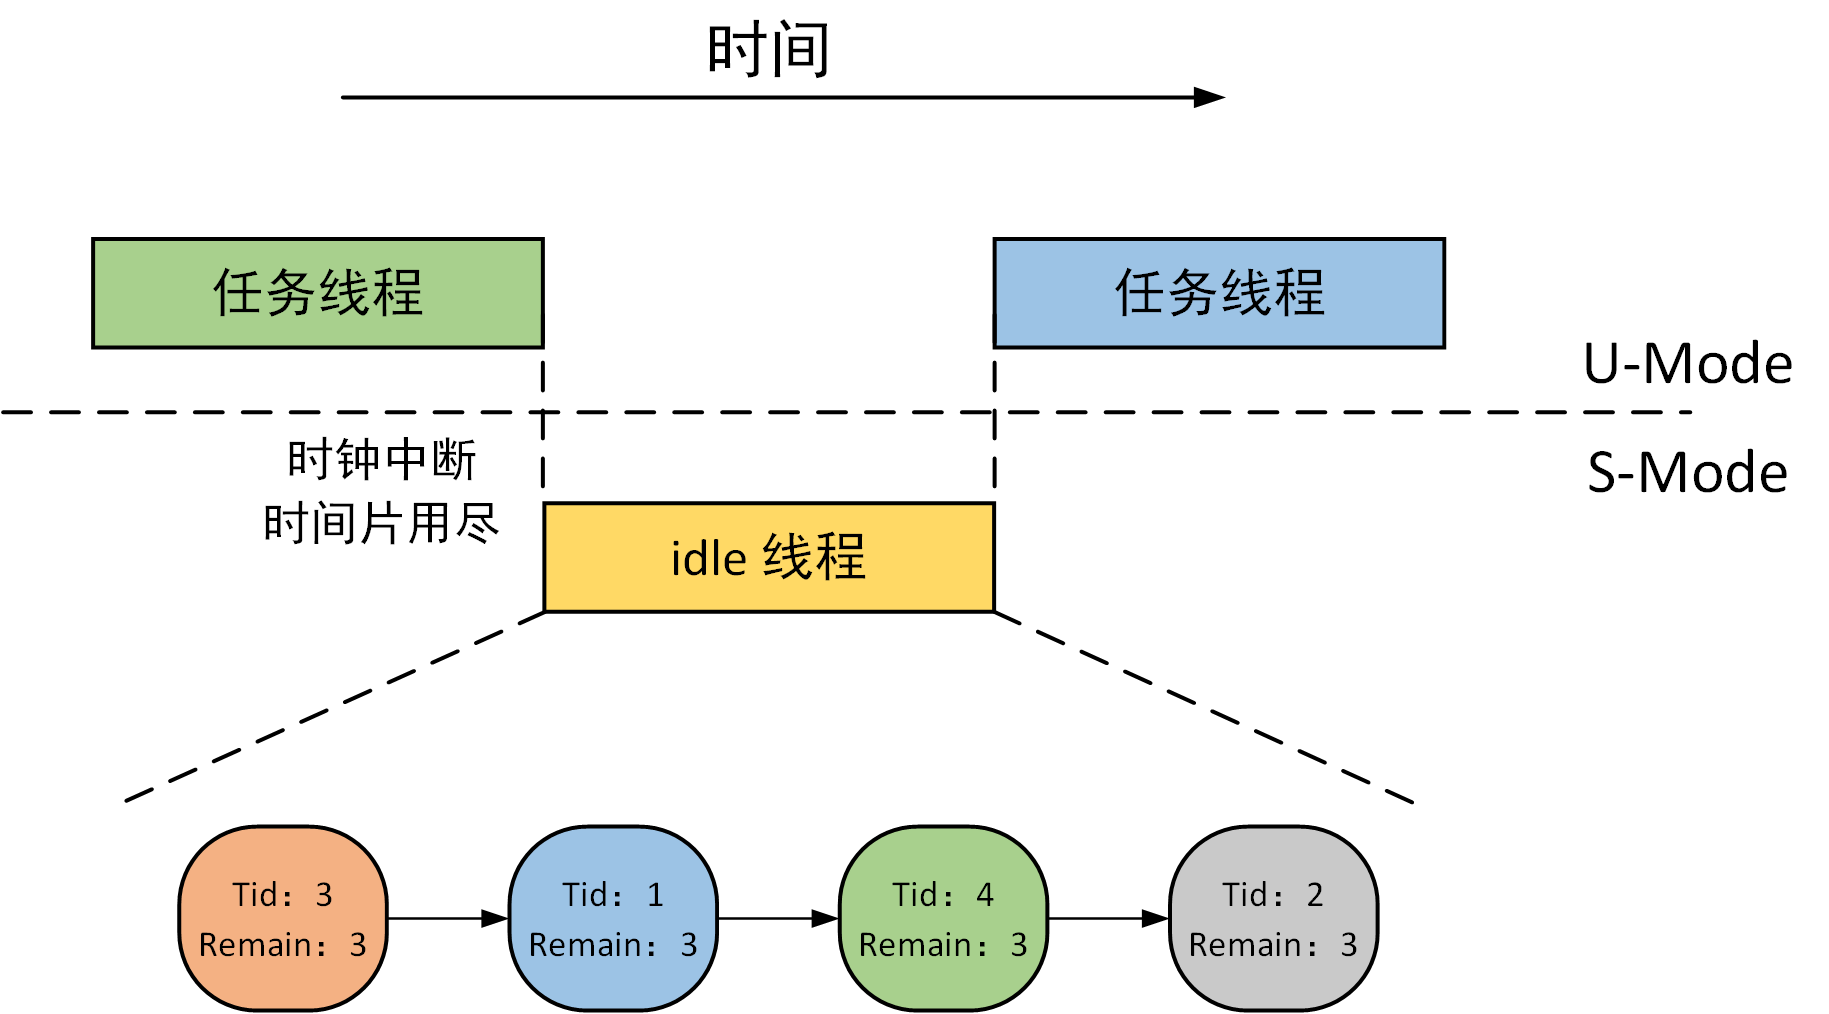
\includegraphics[width=0.75\textwidth]{threadswitch}
	\setlength{\abovecaptionskip}{2pt}
	\caption{线程切换时间线}
	\label{pic:threadswitch}
\end{figure}

在线程用尽时间片,返回到idle线程后,会将上一个线程的资源回收,并防止到线程队列的队尾。随后,idle线程会决策下一个要运行的线程,决策的方式,就是round-robin算法。

Round-Robin算法是一种抢占式调度算法,这意味着如果线程在其拥有的时间片内没有完成任务的话,会被内核打断并让出CPU资源,供下一个线程使用。Round-Robin算法会将时间片平等地分配给所有线程,在较长时间内,每个线程都有均等的机会占用CPU。其大致的思想可大致概括为:

\begin{enumerate}
	\item 将所有的线程存入一个优先队列
	\item 每次调度时都取队首的线程占用CPU
	\item 内核定时去检查正在运行的线程是否用完了时间片,如果没有用完就继续执行,否则就将这个线程放到队尾,执行下一个队首线程。
\end{enumerate}

Moonix使用一个双向环形链表来实现队列,链表的节点按照tid+1作为下标存放在数组中,其中下标0处为Dummy Head,用于快速找到队列头。队列中的元素如代码 \ref{lst:rrinfo} 所示,并不保存实际的线程结构,仅仅以下标记录线程的tid。这种方式侵入性较小,调度器只会向内核返回下一个需要执行的线程的tid,耦合度较低,方便替换和扩展不同的调度算法。

\begin{minipage}[c]{0.95\textwidth}
\begin{lstlisting}[language={C}, caption={线程调度器元素}, label={lst:rrinfo}]
typedef struct
{
	int valid;
	usize time;
	int prev;
	int next;
} RRInfo;
\end{lstlisting}
\end{minipage}
% !Mode:: "TeX:UTF-8"

\chapter{文件系统设计与实现}[filesystem]
\label{chapter:filesystem}

\section{Simple File System}

SimpleFileSystem是一个简单的文件系统,是Unix File System的一个简易实现。Moonix对这个文件系统进行了一定的魔改,但仍然采用这个名字,因为这个文件系统依然足够simple。SimpleFileSystem以下简称SimpleFS。

SimpleFS的总体结构如图 \ref{pic:sfs} 所示,将磁盘分成了数个大小为4096字节的磁盘块。

\begin{figure}[htpb]
	\centering
	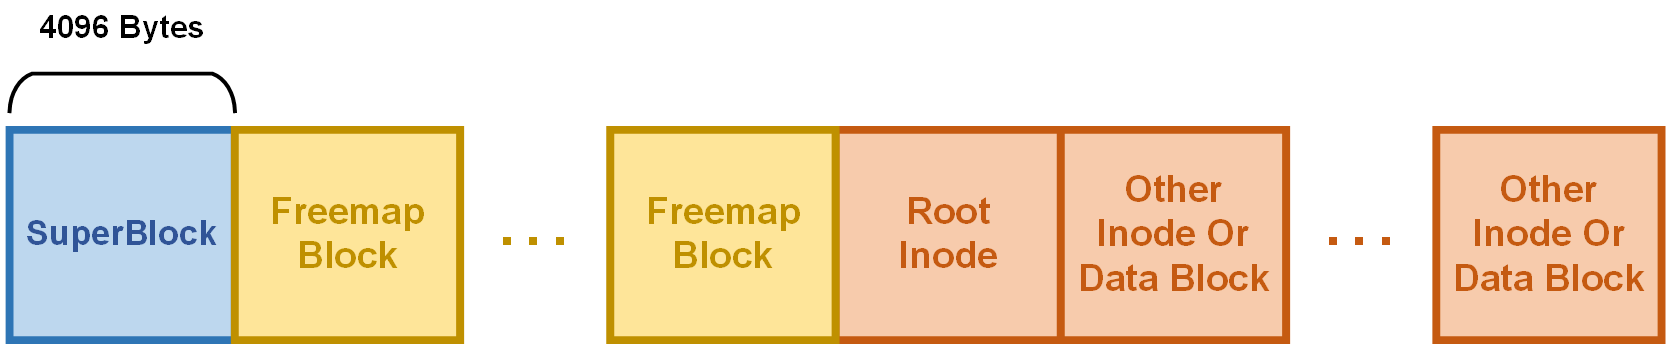
\includegraphics[width=0.85\textwidth]{sfs}
	\setlength{\abovecaptionskip}{2pt}
	\caption{SimpleFS结构}
	\label{pic:sfs}
\end{figure}

一个SimpleFS文件系统的第一块恒为超级块(SuperBlock),它记录了整个文件系统的基本信息,例如总磁盘块数、未使用的磁盘块数、Freemap块个数等。紧随其后的是若干Freemap块,它记录了整个文件系统中磁盘块的占用情况。Freemap块使用一个bit表示一个块,0为未被占用,1为已被占用。通过Freemap块Moonix就可以快速找到空闲可用的磁盘块。Freemap块后面是表示根文件系统的Inode块。SimpleFS也是以树状结构组织文件的,Root即为 “/” 文件夹。Root Inode后就是其他文件的Inode或者数据块,这些块不会做特殊的排序,查找文件需要从根目录开始查找。

\begin{lstlisting}[language={C}, caption={SimpleFS超级块结构}, label={lst:superblock}]
typedef struct {
	uint32 magic;               // 魔数
	uint32 blocks;              // 总磁盘块数
	uint32 unusedBlocks;        // 未使用的磁盘块数
	uint32 freemapBlocks;       // freemap 块数
	uint8 info[32];             // 其他信息
} SuperBlock;
\end{lstlisting}

超级块的结构如代码 \ref{lst:superblock} 所示。第一个字段就是magic number。这个字段恒为 0x4D534653,即ASCII码 “M”、“S”、“F”、“S”。Moonix初始化文件系统时,会首先检查魔数以确定文件系统类型,blocks字段表示这个文件系统一共占用多少个磁盘块。unusedBlocks字段表示这个文件系统目前剩余的空闲磁盘块个数。freemapBlocks表示Freemap块的总个数,这个字段的更重要用处在于推断出Root Inode所在的磁盘块号。最后就是info字段,这是一个字符串,记录了一些其他信息。超级块的实际内容很小,只有48字节,剩余空间由0填充。

\begin{lstlisting}[language={C}, caption={SimpleFS Inode结构}, label={lst:inode}]
typedef struct
{
	uint32 size;                // 文件大小,type 为文件夹时该字段为 0
	uint32 type;                // 文件类型
	uint8 filename[32];         // 文件名称
	uint32 blocks;              // 占据磁盘块个数
	uint32 direct[12];          // 直接磁盘块
	uint32 indirect;            // 间接磁盘块
} Inode;
\end{lstlisting}

一个 Inode 块代表了一个文件或文件夹,结构如代码 \ref{lst:inode} 所示。type字段表示该Inode所代表的文件的类型,可用取值有TYPE\_FILE(普通文件)或TYPE\_DIR(文件夹)。当type取TYPE\_DIR时,size字段为0。并且直接磁盘块和间接磁盘块都是指向存储在该文件夹下的文件的Inode。当type取TYPE\_FILE时,磁盘块指向实际的数据块。当Inode类型为文件夹时,direct[0]和direct[1]分别存储指向当前和指向上一级文件夹的 Inode。

\begin{figure}[htpb]
	\centering
	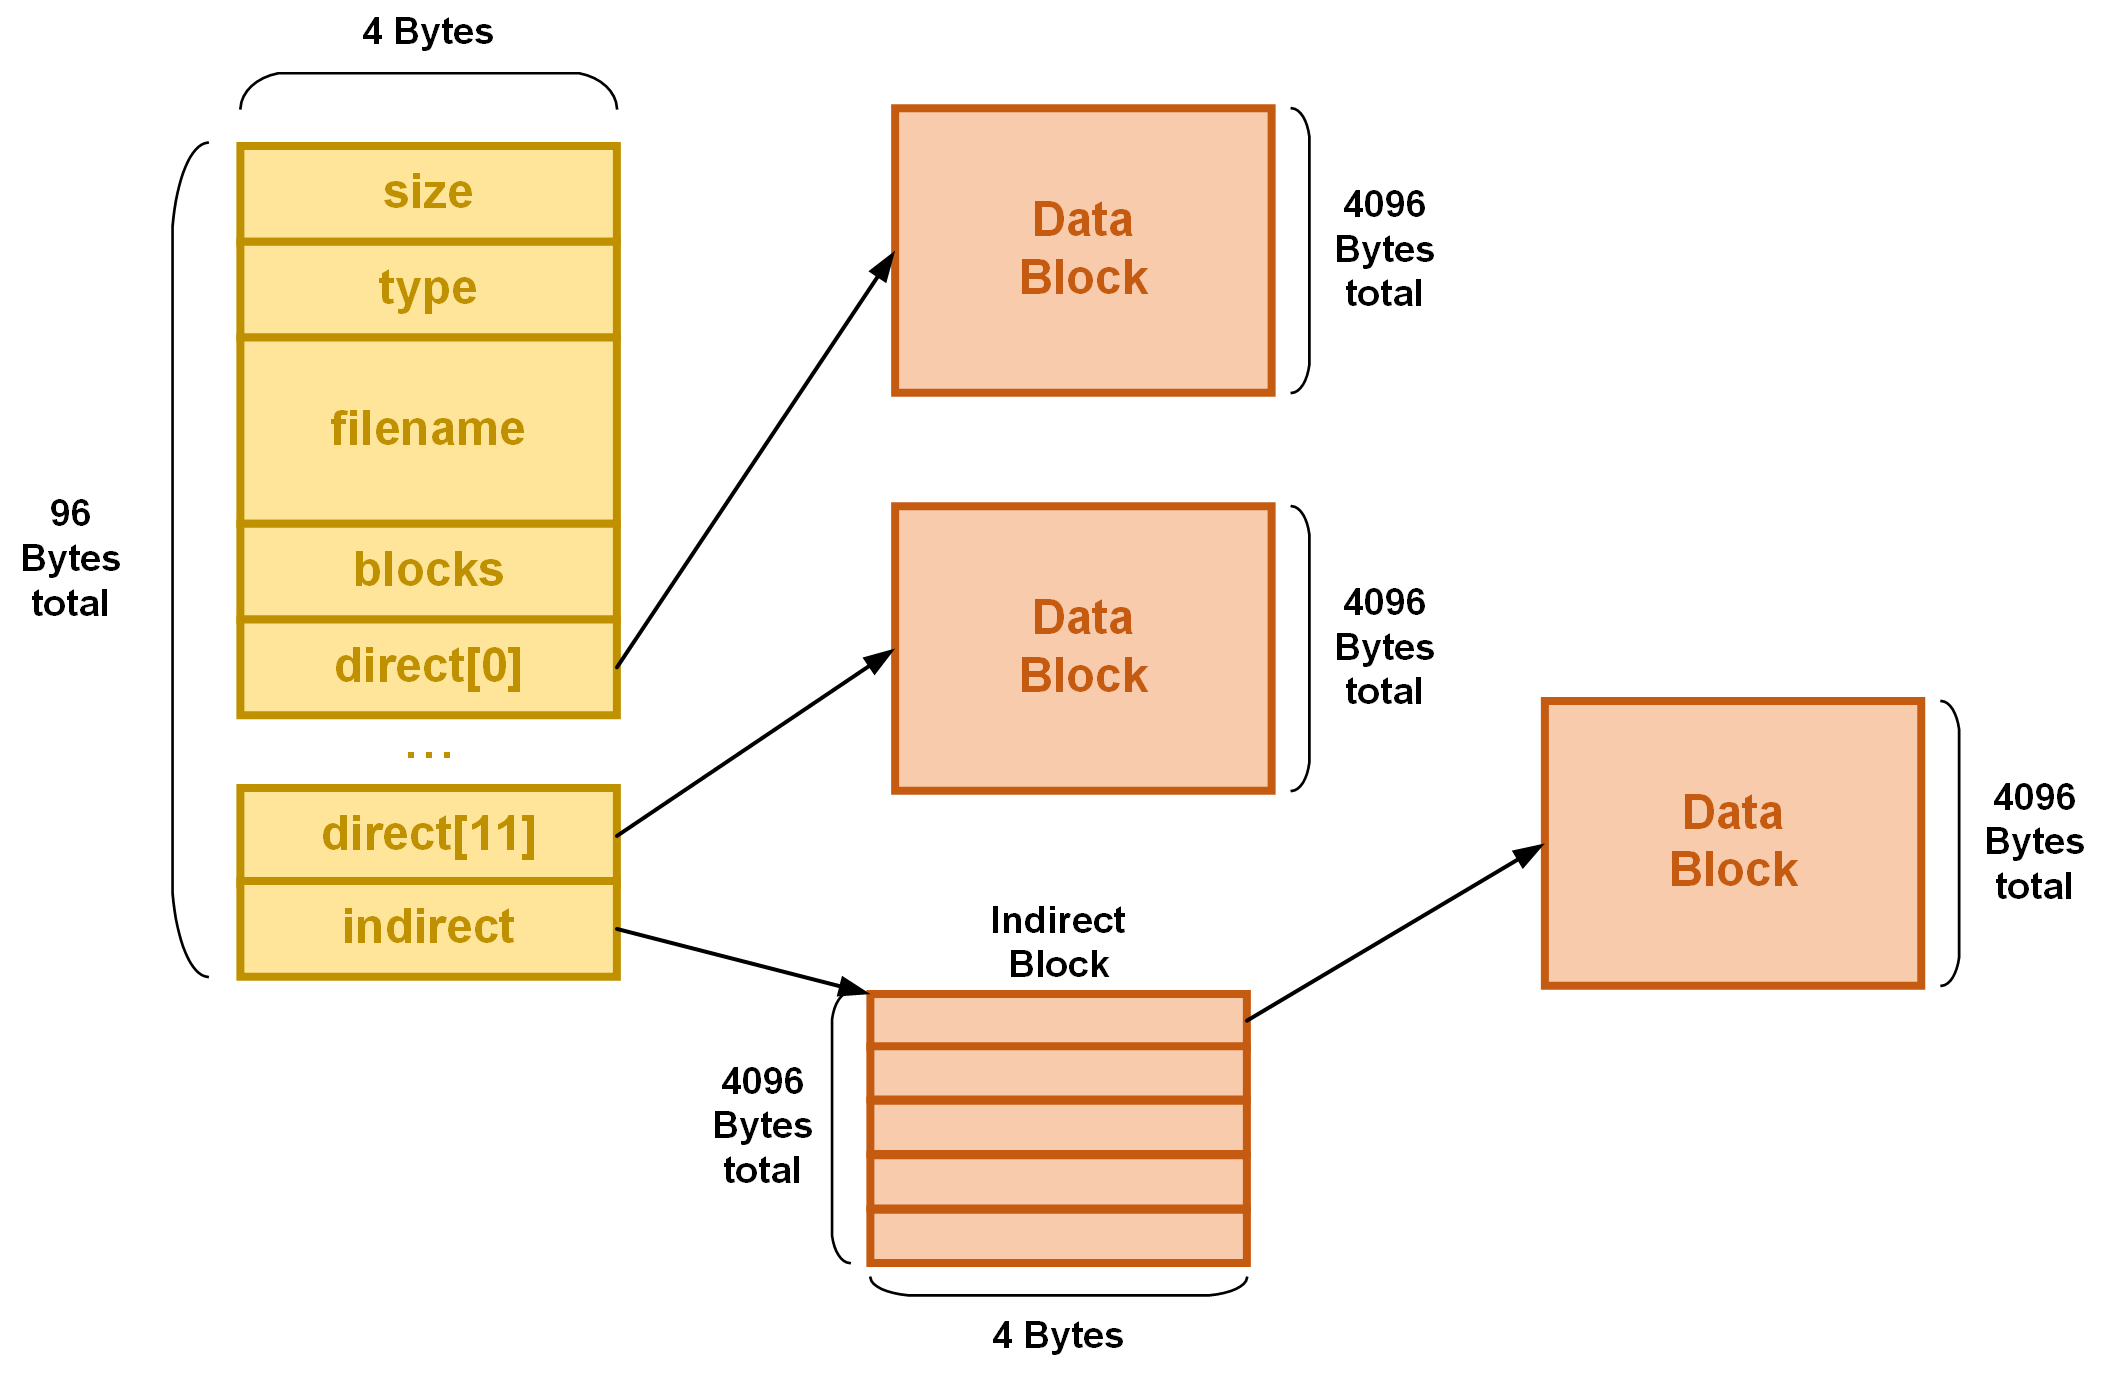
\includegraphics[width=0.70\textwidth]{inode}
	\setlength{\abovecaptionskip}{2pt}
	\caption{Inode直接磁盘块与间接磁盘块}
	\label{pic:inode}
\end{figure}

关于直接磁盘块和间接磁盘块,如图 \ref{pic:inode} 所示。每个Inode块中有一个长度为12的direct数据,如果blocks字段小于等于12,可以直接使用该数组存储磁盘块号,否则,由indirect字段指向一个Indirect Block,在该磁盘块中可以存储更多的磁盘块号。

\section{内核驱动}

目前Moonix没有真正实现文件系统,而是在内核镜像打包时将文件系统镜像直接打包到内核的.text段中,这样Moonix系统在启动时,整个文件系统就已经存在于内存之中了,.text段中的文件系统前后都有全局符号标记,使得内核可以直接寻找到文件系统的开头。

Moonix操作系统在启动初始化时,最后一步就是去初始化文件系统,并从文件系统中获取shell可执行文件,并加载执行。文件系统的初始化工作比较简单,由于本文件系统的特性,内核只需要根据全局符号,获取到文件系统的开头字节,读入超级块解析文件系统的基本信息,寻找并缓冲root目录的Inode即可。

文件系统驱动中,lookup函数是一个比较核心的函数。lookup函数将传入的Inode作为当前目录,从当前目录下根据路径查找文件。例如,若当前目录为/usr,传入./hello和hello甚至../usr/hello都可以找到可执行文件hello。如果传入的路径以/开头,函数会忽略当前路径而从根目录下开始查找。如果传入的Inode为null,函数也会从根目录开始查找。函数会根据路径分割出需要在当前目录下查找的文件或文件夹名称,并递归调用lookup函数进一步搜索。

另一个比较核心的函数,是readall函数。readall函数传入一个文件类型的Inode。这个函数将该Inode所代表的文件数据全部拷贝到字节数组中。这个函数主要用于操作系统或者用户在执行某个可执行文件时,获取到Inode之后,需要将这个Inode所表示的文件拷贝到内核中。传入的字节数组通常是动态内存分配得到的,在操作系统解析并获取映射各个段之后,这个数组会被内核回收。
% !Mode:: "TeX:UTF-8"

\chapter{shell的实现}[shell]
\label{chapter:shell}

\section{模块概述}

Moonix操作系统在初始化阶段,做的最后一件事,就是加载文件系统的 /bin/sh可执行文件,并将其作为用户进程运行起来。

/bin/sh是一个执行在用户态的shell,是用户和Moonix交互的唯一途径。用户可以直接在shell中键入文件系统上可执行文件的路径,操作系统会将这个文件加载到内核并解析映射,并执行这个可执行文件,在该文件执行结束后,会再切换会shell进程,等待用户的其他命令。除了执行可执行文件外,shell还内建了几个简单的命令,如cd、ls、pwd等,方便用户可以穿梭在文件夹中,方便查看与执行文件。

\section{用户程序的加载与运行}

本节以shell程序为例。

在线程初始化的最后部分,Moonix操作系统从文件系统中加载 /bin/sh,并将其初始化为用户进程,添加到进程调度中。如代码 \ref{lst:initshell} 所示。

\begin{minipage}[c]{0.95\textwidth}
\begin{lstlisting}[language={moonix}, caption={Moonix加载shell}, label={lst:initshell}]
/* 启动终端 */
Inode *shInode = lookup(0, "/bin/sh");
char *buf = kalloc(shInode->size);
readall(shInode, buf);
Thread t = newUserThread(buf);
kfree(buf);
addToCPU(t);
\end{lstlisting}
\end{minipage}

Moonix首先使用文件系统的lookup接口,从文件系统中获取到了保存/bin/sh文件信息的Inode,并根据Inode中记录的文件大小,使用动态内存分配,在堆空间中开辟了一块缓存buf。随后使用文件系统的readall接口,从文件系统中读取了程序的数据文件,并保存到了buf中。随后根据这个文件构建了一个用户进程,添加到CPU的进程调度中。

构建用户进程的关键点在于解析一个完整的程序文件,这个程序文件是ELF格式的可执行文件。Moonix首先根据ELF头的信息,找到程序头表相对于ELF文件开头的偏移,进而找到文件头表。文件头中的p\_type描述了段类型,Moonix只需要将LOAD类型的段装载进内存即可。内核将代码或数据复制进物理内存之后,需要在页表中映射到虚拟地址空间,页表项的权限需要根据程序头中的p\_flags段权限转化。ELF头的entry字段记录了程序入口的虚拟地址。

Moonix构建用户进程时,除去要映射用户程序的代码和数据到虚拟地址空间,还需要将内核映射到虚拟地址空间中,以保证用户进程在发起环境调用时,进程进入S-Mode,能够顺利进入内核处理调用。于是在构建用户进程时,解析ELF文件之前,Moonix首先会填充一个已经映射好内核的页表,随后在这个页表的基础上继续映射程序私有的代码数据。

\section{用户态环境调用}

shell是一个U-Mode进程,而内核运行在S-Mode下。通常,一个U-Mode进程的能力十分有限,大部分能力都需要依赖操作系统功能,甚至输出一个字符到屏幕上,都必须通过操作系统。U-Mode环境与内核唯一的沟通渠道,就是通过环境调用的方式。

RISC-V规范规定,环境调用的调用号通过a7寄存器传递,参数通过a1、a2和a3寄存器,处理结果的返回值通过a0寄存器传递。如代码 \ref{lst:shell} 所示,Moonix通过内联汇编的方式,执行ecall指令,并在执行指令之前填充参数和调用号寄存器。

当一个U-Mode环境调用发生时,Moonix内核会接收到一个系统中断,中断类型是USER\_ENV\_CALL。Moonix随后会从a7寄存器中取出中断调用号,从a1、a2、a3寄存器中取出参数,根据调用号的类型进行不同的处理,并将返回值写入a0寄存器中,结束这次中断处理。

当shell通过EXEC环境调用执行某个可执行文件时,由于此时shell也在运行状态,由于被执行的进程和shell处于并发执行状态,两个进程的输出可能会混杂到一起。所以在执行EXEC系统调用时,Moonix会挂起发起系统调用的线程,使得shell进入休眠状态,直到被执行的进程结束,shell进程才会被重新调度。

\begin{minipage}[c]{0.95\textwidth}
\begin{lstlisting}[language={moonix}, caption={U-Mode环境调用}, label={lst:shell}]
typedef enum {
	Shutdown = 13,
	LsDir = 20,
	CdDir = 21,
	Pwd = 22,
	Open = 56,
	Close = 57,
	Read = 63,
	Write = 64,
	Exit = 93,
	Exec = 221,
} SyscallId;

#define sys_call(__num, __a0, __a1, __a2, __a3)                          \
({                                                                  \
	register unsigned long a0 asm("a0") = (unsigned long)(__a0);    \
	register unsigned long a1 asm("a1") = (unsigned long)(__a1);    \
	register unsigned long a2 asm("a2") = (unsigned long)(__a2);    \
	register unsigned long a3 asm("a3") = (unsigned long)(__a3);    \
	register unsigned long a7 asm("a7") = (unsigned long)(__num);   \
	asm volatile("ecall"                                            \
	: "+r"(a0)                                          \
	: "r"(a1), "r"(a2), "r"(a3), "r"(a7)                         \
	: "memory");                                        \
	a0;                                                             \
})
\end{lstlisting}
\end{minipage}
\backmatter
% !Mode:: "TeX:UTF-8" 
\begin{conclusions}

学位论文的结论作为论文正文的最后一章单独排写,但不加章标题序号。

结论应是作者在学位论文研究过程中所取得的创新性成果的概要总结,不能与摘要混为一谈。博士学位论文结论应包括论文的主要结果、创新点、展望三部分,在结论中应概括论文的核心观点,明确、客观地指出本研究内容的创新性成果(含新见解、新观点、方法创新、技术创新、理论创新),并指出今后进一步在本研究方向进行研究工作的展望与设想。对所取得的创新性成果应注意从定性和定量两方面给出科学、准确的评价,分(1)、(2)、(3)…条列出,宜用“提出了”、“建立了”等词叙述。

\end{conclusions}
   % 结论
\bibliographystyle{hithesis} %如果没有参考文献时候
\bibliography{reference}

\authorization %授权
% % \authorization[saomiao.pdf] %添加扫描页的命令,与上互斥
% !Mode:: "TeX:UTF-8"
\begin{acknowledgements}

Moonix操作系统和本论文是在刘国军老师的指导下完成的。刘国军老师教授的操作系统课程,使我对操作系统的设计与实现产生了浓厚的兴趣,并最终促成的我的选题。在项目进行过程中,刘国军老师渊博的专业知识和悉心的指导,使得我能够最终完成这个项目。在此,谨向刘国军老师致以最诚挚的谢意。

感谢大学期间所有教过我的老师们,你们严谨的治学精神、渊博的专业知识,培养了我对计算机科学浓厚的兴趣,非常感谢。

感谢我的女朋友。很多时候,我都疲于学业和工作,没法常伴她左右,她也不曾有一丝怨言。Moonix操作系统就是以她的名字命名的,以表达我对她的谢意。这一点我一直没好意思告诉刘国军老师。

感谢我的父母给予我无私的关心和照顾,没有你们的照顾和支持,就不会有我的今天,我永远无法回报你们对我的爱,所以我希望能顺利完成学业,给你们一点欣慰。

感谢所有帮助过我的老师、同学和朋友,没有你们的帮助,就没有我今天的成绩。

感谢字节跳动的同事们,本论文是在字节跳动实习期间完成的,感谢他们对于我摸鱼写论文和频繁请假的包容。你们开放谦逊、坦诚清晰的字节范儿,使得我对未来的工作充满的期待,很荣幸能和你们成为同事。

最后再次感谢所有帮助过我的老师、家人、同学和朋友们!

\end{acknowledgements}
 %致谢
%\begin{appendix}%附录
%\input{back/appendix1}
%\end{appendix}

\end{document}